%%%%%%%%%%%%%%%%%%%%%%%%%%%%%%%%%%%%%%%%%%%%%%%%%%%%%%%%%%%%%%%%%%%%%%%%%%%%%%%%
%% Plantilla de memoria en LaTeX para la ETSIT - Universidad Rey Juan Carlos
%%
%% Por Gregorio Robles <grex arroba gsyc.urjc.es>
%%     Grupo de Sistemas y Comunicaciones
%%     Escuela Técnica Superior de Ingenieros de Telecomunicación
%%     Universidad Rey Juan Carlos
%% (muchas ideas tomadas de Internet, colegas del GSyC, antiguos alumnos...
%%  etc. Muchas gracias a todos)
%%
%% La última versión de esta plantilla está siempre disponible en:
%%     https://github.com/gregoriorobles/plantilla-memoria
%%
%% Para obtener PDF, ejecuta en la shell:
%%   make
%% (las imágenes deben ir en PNG o JPG)

%%%%%%%%%%%%%%%%%%%%%%%%%%%%%%%%%%%%%%%%%%%%%%%%%%%%%%%%%%%%%%%%%%%%%%%%%%%%%%%%
	
\documentclass[a4paper, 12pt]{book}
%\usepackage[T1]{fontenc}

\usepackage[a4paper, left=2.5cm, right=2.5cm, top=3cm, bottom=3cm]{geometry}
\usepackage{times}
\usepackage[utf8]{inputenc}
%\usepackage[spanish]{babel} % Comenta esta línea si tu memoria es en inglés
\usepackage{url}
%\usepackage[dvipdfm]{graphicx}
\usepackage{graphicx}
\usepackage{float}  %% H para posicionar figuras
\usepackage[nottoc, notlot, notlof, notindex]{tocbibind} %% Opciones de índice
\usepackage{latexsym}  %% Logo LaTeX
\usepackage{subfig}
\usepackage{hyperref}
\hypersetup{
    colorlinks,
    citecolor=red,
    filecolor=red,
    linkcolor=red,
    urlcolor=red
}
\usepackage{listings}

\title{Master's Thesis}
\author{David Moreno Lumbreras}

\renewcommand{\baselinestretch}{1.5}  %% Interlineado

\begin{document}

%\renewcommand{\refname}{Bibliografía}  %% Renombrando
\renewcommand{\appendixname}{Appendix}

%%%%%%%%%%%%%%%%%%%%%%%%%%%%%%%%%%%%%%%%%%%%%%%%%%%%%%%%%%%%%%%%%%%%%%%%%%%%%%%%
% PORTADA

\begin{titlepage}
\begin{center}
\begin{tabular}[c]{c c}
%\includegraphics[bb=0 0 194 352, scale=0.25]{logo} &

\includegraphics[scale=0.25]{img/logo_vect.png} &
\begin{tabular}[b]{l}
\Huge
\textsf{UNIVERSIDAD} \\
\Huge
\textsf{REY JUAN CARLOS} \\
\end{tabular}
\\
\end{tabular}

\vspace{3cm}

\Large
Máster Universitario en Ingeniería de Telecomunicación

\vspace{0.4cm}

\large
Curso Académico 2018/2019

\vspace{0.8cm}

Trabajo Fin de Máster

\vspace{2.5cm}

\LARGE
VBoard

\large
Web dashboards in 3D and VR

\vspace{4cm}

\large
Autor : David Moreno Lumbreras\\
Tutor : Dr. Jesús M. González Barahona
\end{center}
\end{titlepage}

\newpage
\mbox{}
\thispagestyle{empty} % para que no se numere esta pagina


%%%%%%%%%%%%%%%%%%%%%%%%%%%%%%%%%%%%%%%%%%%%%%%%%%%%%%%%%%%%%%%%%%%%%%%%%%%%%%%%
%%%% Dedicatoria

\chapter*{}
\pagenumbering{Roman} % para comenzar la numeracion de paginas en numeros romanos
\begin{flushright}
\textit{Dedicatoria
}
\end{flushright}

%%%%%%%%%%%%%%%%%%%%%%%%%%%%%%%%%%%%%%%%%%%%%%%%%%%%%%%%%%%%%%%%%%%%%%%%%%%%%%%%
%%%% Agradecimientos

\chapter*{Acknowledgment}
%\addcontentsline{toc}{chapter}{Agradecimientos} % si queremos que aparezca en el índice
\markboth{Acknowledgment}{Acknowledgment} % encabezado 

Agradecimientos

And finally, these are two of my favourite quotes:\\ 

\textit{"Caer esta permitido, levantarse es obligatorio"}\\
\textit{"El final de un viaje es siempre el principio de otro"}


%%%%%%%%%%%%%%%%%%%%%%%%%%%%%%%%%%%%%%%%%%%%%%%%%%%%%%%%%%%%%%%%%%%%%%%%%%%%%%%%
%%%% Resumen en inglés

\chapter*{Abstract}
%\addcontentsline{toc}{chapter}{Abstract} % si queremos que aparezca en el índice
\markboth{ABSTRACT}{ABSTRACT} % encabezado
Abstract

%%%%%%%%%%%%%%%%%%%%%%%%%%%%%%%%%%%%%%%%%%%%%%%%%%%%%%%%%%%%%%%%%%%%%%%%%%%%%%%%
%%%% Resumen

\chapter*{Resumen}
%\addcontentsline{toc}{chapter}{Resumen} % si queremos que aparezca en el índice
\markboth{RESUMEN}{RESUMEN} % encabezado

Resumen

%%%%%%%%%%%%%%%%%%%%%%%%%%%%%%%%%%%%%%%%%%%%%%%%%%%%%%%%%%%%%%%%%%%%%%%%%%%%%%%%
%%%%%%%%%%%%%%%%%%%%%%%%%%%%%%%%%%%%%%%%%%%%%%%%%%%%%%%%%%%%%%%%%%%%%%%%%%%%%%%%
% ÍNDICES %
%%%%%%%%%%%%%%%%%%%%%%%%%%%%%%%%%%%%%%%%%%%%%%%%%%%%%%%%%%%%%%%%%%%%%%%%%%%%%%%%

% Las buenas noticias es que los índices se generan automáticamente.
% Lo único que tienes que hacer es elegir cuáles quieren que se generen,
% y comentar/descomentar esa instrucción de LaTeX.

%%%% Índice de contenidos
\tableofcontents 
%%%% Índice de figuras
\cleardoublepage
%\addcontentsline{toc}{chapter}{Lista de figuras} % para que aparezca en el indice de contenidos
\listoffigures % indice de figuras
%%%% Índice de tablas
%\cleardoublepage
%\addcontentsline{toc}{chapter}{Lista de tablas} % para que aparezca en el indice de contenidos
%\listoftables % indice de tablas

%%%%%%%%%%%%%%%%%%%%%%%%%%%%%%%%%%%%%%%%%%%%%%%%%%%%%%%%%%%%%%%%%%%%%%%%%%%%%%%%
%%%%%%%%%%%%%%%%%%%%%%%%%%%%%%%%%%%%%%%%%%%%%%%%%%%%%%%%%%%%%%%%%%%%%%%%%%%%%%%%
% INTRODUCCI�N %
%%%%%%%%%%%%%%%%%%%%%%%%%%%%%%%%%%%%%%%%%%%%%%%%%%%%%%%%%%%%%%%%%%%%%%%%%%%%%%%%

\cleardoublepage
\chapter{Introduction}
\label{sec:intro} % etiqueta para poder referenciar luego en el texto con ~\ref{sec:intro}
\pagenumbering{arabic} % para empezar la numeraci�n de p�gina con n�meros

In this chapter we will describe the problem description and introduce the project objectives and its context, in order to clarify its basis before to dive into the technical details.

\section{Problem description}
\label{sec:probdescr}

Nowadays, companies have a big amount of data (sells, products, incomes, costumers), therefore, the visualization of these displays a very important role in the business process. This data must be understandable for its subsequent analysis or usage. Our brain interprets better and quicker the information when it's received through a graphic process. Through visual communication, a bunch of complex data makes easier to understand. These are usually shown as graphics, either circular, lineal, in barcodes, etc. This project is based in the visualization of this data storage in a different way, a dashboard with different types of chars but in 3D and Virtual Reality. This way of visualization is unexploited. There aren't applications to fulfill this kind of data visualization. That's why this project would work in something innovative inside open source software engineering.

There are tools like Kibana, Grafana or Freeboard that allow showing the data that come from databases from different types of visualizations and dashboards. This project will build a interface from scratch using Three.js and A-frame as 3D rendering engine and using ElasticSearch as the database.

This project, called VBoard, is a tool with open source software license that allows to visualize and explore data that comes from ElasticSearch. ElasticSearch is a NoSQL database that allows to index a big amount of data, it can make searches and analyse such data in real time. Data can be visualize through VBoard in a little exploited way, making visualizations in 3D (piechart, lineal, bars with 3 axis, bubbles, etc.) and after, it can be include those visualizations in the same dashboard with the aim of watching the data in different ways of visualization, always in the 3D scope with the possibility of "enter" the dashboard with the Virtual Reality.

These are not applications that allow this type of data visualization. Is because of that, that it's been chosen as a project the creation of an application that allows visualize data in the 3D scope, and afterwards, navigate with Virtual Reality into it.

\section{Main Objective and Requirements}
\label{sec:mainobj}


This project's main aim is the development of a complex system of data visualization in 3D and VR. It's been chosen for this project the creation of a web application. This project should show the data of the ElasticSearch database in a 3D way relating the fields that have been previously selected. Finally, the next goal is to integrate it in a dashboard with other data visualizations and add the possibility to navigate in Virtual Reality into it.

Inside this main aim, there are a number of sub-goals:

\begin{itemize}
\item Analysis and choice of visualization’s library: Study and analysis of different visualization’s libraries of 3D and VR so, afterwards, a library that follows the requirements for the development of the project can be chosen. This can be reached through the creation and modification of little examples of each library according to its API's.
\item Analysis and choice of web development framework: Estudio de los diferentes frameworks de desarrollo que hay para realizar aplicaciones web y posterior elección de aquel que se ajuste más a los requisitos y cumpla con la funcionalidades acordadas. Es de imporancia que este framework de desarrollo permita la conexión al servicio externo ElasticSearch ya que va a ser la base de datos.
\item Búsqueda y desarrollo de API's: para el desarrollo del proyecto, va a ser necesario el uso y desarrollo de distintas API's Javascript con el fin de albergar todas las funcionalidades requeridas para el proyecto. Se requerirá un previo de estudio de estas API's y un posterior desarrollo de nuevas API's para completar aquellas que no cumplen con todos los requerimientos.
\item Desarrollo de una interfaz simple y de facil uso: con el fin de que esta plataforma sea fácilmente usable, hay que realizar un concienzado desarrollo de la parte gráfica para que cualquier persona sin importar el nivel de conocimiento técnico, sea capaz de utilizar la aplicación por completo sin problemas. Para ello puede complementarse el desarrollo con una guía de usuario y ejemplos mediante videos, gifs o capturas.
\item Definir objetos de la plataforma e índices en ElasticSearch para su posterior guardado: para poder mantener un estado de las visualizaciones y dashboards que se vayan creando, es necesario definir que tipos de objetos se van a guardar y un índice especial en ElasticSearch para esta aplicación. Dentro de este índice se guardará en tipos o documentos las visualaciones o dashboards, que serán los objetos. Además la aplicación debe ser capaz de crear/editar este índice de manera autónoma, como por ejemplo, crear el índice si no existe, actualizar documentos, etc.
\item Vista de sólo dashboard e integrar VR: una vez la aplicación esté completa, hay que permitir la visualización de los dashboards en distintas e independientes URLs, de esta manera solo se verá el dashboard aislado de la interfaz de la aplicación, así los datos pueden ser rápidamente enseñables sin necesidad de pasar por el proceso de carga o interacción con la interfaz. Además, dentro de esta vista debe de haber algún modo capaz de activar la VR para poder observar el dashboard con un dispositivo VR (e.g. un Smarthpone).
\item Crear imagen Docker: para que esta aplicación se extienda y pueda ser fácilmente instabalble y desplegable en cualqueir máquina, se construirá una imagen docker de la aplicación para que una vez creado un contenedor, el servicio VBoard se haya desplegado y se pueda acceder inmediatamente. Esta imagen deberá estar disponible en Dockerhub de tal manera que cualquier persona pueda descargarla. Además, debe de haber un lugar en el repositorio con información de estas imágenes así como ejemplos de como desplegarla.
\end{itemize}

\section{Software Availability}
\label{sec:softavail}

The project is hosted in the web-based Git repository hosting service GitHub, under open source software license. It has a web page of presentation where more information and details of the project are provided to the user. Inside the repository, where project's software is hosted, there's documentation like the installation steps and the user and usage manual.

Furthermore, there is a Docker image of the application in order to install and deploy it easily, the image is hosted in Dockerhub from Docker (platform where users/organizations upload their images) and inside the repository, there is also a guide of how to deploy VBoard via docker and docker-compose with some examples. 

\begin{itemize}
\item Project page: \url{https://dlumbrer.github.io/VBoard/}
\item GitHub Repository: \url{https://github.com/dlumbrer/VBoard}
\item Dockerhub: \url{https://hub.docker.com/r/dlumbrer/vboard/}
\item Docker deployment guide: \url{https://github.com/dlumbrer/VBoard/tree/docker}
\end{itemize}

%%%%%%%%%%%%%%%%%%%%%%%%%%%%%%%%%%%%%%%%%%%%%%%%%%%%%%%%%%%%%%%%%%%%%%%%%%%%%%%%
%%%%%%%%%%%%%%%%%%%%%%%%%%%%%%%%%%%%%%%%%%%%%%%%%%%%%%%%%%%%%%%%%%%%%%%%%%%%%%%%
% ESTADO DEL ARTE %
%%%%%%%%%%%%%%%%%%%%%%%%%%%%%%%%%%%%%%%%%%%%%%%%%%%%%%%%%%%%%%%%%%%%%%%%%%%%%%%%


\chapter{Context and Used technologies}

In this chapter we will take a look to the open source software philosophy and the most important technologies used to make this project, we start with a general description of the technology and then we describe how we use it in the project. Now, we will talk about the different technologies used in this project: This project is developed in JavaScript with part of HTML5 and CSS and for the development of this project we will use different modules that have been imported through NPM; Moreover, in order to make a strong and modern web application, it has been used the JavaScript framework AngularJS; the ElasticSearch database is based on NodeJS.

\section{HTML5}
\label{sec:html5}
\subsection{General description}
\label{sec:html5gd}
HTML5 is a markup language used for structuring and presenting content on the World Wide Web. It was finalized, and published, on 28 October 2014 by the World Wide Web Consortium (W3C) This is the fifth revision of the HTML standard since the inception of the World Wide Web. The previous version, HTML 4, was standardized in 1997.

Its core aims are to improve the language with support for the latest multimedia while keeping it easily readable by humans and consistently understood by computers and devices (web browsers, parsers, etc.). HTML5 is intended to subsume not only HTML 4, but also XHTML 1 and DOM Level 2 HTML.

In particular, HTML5 adds many new syntactic features. These include the new video, audio and canvas elements, as well as the integration of scalable vector graphics (SVG) content (replacing generic object tags) and MathML for mathematical formulas. These features are designed to make it easy to include and handle multimedia and graphical content on the web without having to resort to proprietary plugins and APIs. Other new page structure elements, such as main, section, article, header, footer, aside, nav and figure, are designed to enrich the semantic content of documents. New attr	ibutes have been introduced, some elements and attributes have been removed and some elements, such as a, cite and menu> have been changed, redefined or standardized. The APIs and Document Object Model (DOM) are no longer afterthoughts, but are fundamental parts of the HTML5 specification.HTML5 also defines in some detail the required processing for invalid documents so that syntax errors will be treated uniformly by all conforming browsers and other user agents.
\subsection{In this project}
\label{sec:html5itp}
As we said in the previous subsection, HTML5 adds the new syntactic feature known as Canvas, allowing us to render dynamic graphics and animations on our web pages. Almost all web browsers supports Canvas today.
VisJS use a div to fill it with a canvas. The canvas is where the social network is rendered.
\lstset{language=Java, breaklines=true, basicstyle=\footnotesize}
\begin{lstlisting}[frame=single]
   // attach div element to variable to contain the render
   var container = document.getElementById( 'mynetwork' );
   // VisJS with this sentence build and render the canvas into the 'container'
   var network = new visN.Network(container, data, options);
\end{lstlisting}
Where the container is the div with 'mynetwork' tag (for example).

\section{JavaScript}
\label{sec:js}
JavaScript is a high-level, dynamic, untyped, and interpreted programming language.It has been standardized in the ECMAScript language specification. Alongside HTML and CSS, it is one of the three essential technologies of World Wide Web content production; the majority of websites employ it and it is supported by all modern Web browsers without plug-ins.JavaScript is prototype-based with first-class functions, making it a multi-paradigm language, supporting object-oriented,imperative, and functional programming styles.It has an API for working with text, arrays, dates and regular expressions, but does not include any I/O, such as networking, storage, or graphics facilities, relying for these upon the host environment in which it is embedded. JavaScript have this main features:

\begin{itemize}  
\item \underline{Imperative and structured}: 
JavaScript supports much of the structured programming syntax from C (e.g., if statements, while loops, switch statements, do while loops, etc.). One partial exception is scoping: JavaScript originally had only function scoping with var.
\item \underline{Dynamic}:
As with most scripting languages, JavaScript is dynamically typed; a type is associated with each value, rather than just with each expression. JavaScript includes an eval function that can execute statements provided as strings at run-time.
\item \underline{Prototype-based (Object-oriented)}:
JavaScript is almost entirely object-based. In JavaScript, an object is an associative array, augmented with a prototype (see below); each string key provides the name for an object property, and there are two syntactical ways to specify such a name: dot notation (obj.x = 10) and bracket notation (obj['x'] = 10). A property may be added, rebound, or deleted at run-time. JavaScript has a small number of built-in objects, including Function and Date.
\item \underline{Functional}:
A function is first-class; a function is considered to be an object. As such, a function may have properties and methods, such as .call() and .bind(). JavaScript also supports anonymous functions.
\end{itemize}
\underline{Syntax examples}:
\begin{lstlisting}[frame=single]
var x; // defines the variable x, the special value 'undefined' (not to be confused with an undefined value) is assigned to it by default
var y = 2; // defines the variable y and assigns the value of 2 to it

//A simple recursive function:
function factorial(n) {
    if (n == 0) {
        return 1;
    }
    return n*factorial(n - 1);
}

//Anonymous function (or lambda) syntax and closure example:
var displayClosure = function() {
    var count = 0;
    return function () {
        return ++count;
    };
}
var inc = displayClosure();
inc(); // returns 1
inc(); // returns 2
inc(); // returns 3
\end{lstlisting}
\subsection{In this project}

Is have been used JavaScript for all the scripts in the project, and also, all the libraries we have included are written in JavaScript, these libraries are described in detail in the following sections.  

 \section{Kibana}
\label{sec:kibana}
Kibana is an open source analytics and visualization platform designed to work with Elasticsearch. We use Kibana to search, view, and interact with data stored in Elasticsearch indices. We can easily perform advanced data analysis and visualize our data in a variety of charts, tables, and maps.

Kibana makes it easy to understand large volumes of data. Its simple, browser-based interface enables you to quickly create and share dynamic dashboards that display changes to Elasticsearch queries in real time. 	Setting up Kibana is a snap. We can install Kibana and start exploring your Elasticsearch indices in minutes (no code, no additional infrastructure required).

Kibana should be configured to run against an Elasticsearch node of the same version. This is the officially supported configuration.

\subsection{Index(es) Setting}
When Kibana starts up for the first time, you will be asked to configure an index pattern. The first important step is to select whether you want to handle time-based events which data-set contains a timestamp in each document or if you want to work with "static" data. In Elasticsearch it is common to store time-based events in multiple indexes to facilitate search and allow for memory optimization.

For all time-based data, you can select the time span, that you want to analyze in the current view at the top right of the window. There are multiple ways to get to the documents you are interested in: Either use the Quick tab to quickly select a date range like today or Last 1 hour or use the relative and absolute tabs to specify which time spans you want to look at.

\begin{figure}[H]
  \centering
  \includegraphics[width=16cm, keepaspectratio]{img/context/timespan}
  \caption{Time span selection}
  \label{fig:timespan}
\end{figure}


\subsection{Pages in Kibana}
At the left of the page, Kibana shows the main navigation, which will give you access to the three main pages in Kibana: Discover, Visualize, Dashboard. Below, we give a short overview of the purposes of those sections.


\begin{figure}[H]
  \centering
  \includegraphics[width=2.5cm, keepaspectratio]{img/context/PagesKibana}
  \caption{List of Pages}
  \label{fig:pageskibana}
\end{figure}

\subsubsection{Discover}
You can interactively explore your data from the Discover page. You have access to every document in every index that matches the selected index pattern. You can submit search queries, filter the search results, and view document data. You can also see the number of documents that match the search query and get field value statistics. If a time field is configured for the selected index pattern, the distribution of documents over time is displayed in a histogram at the top of the page.

\subsubsection{Visualize}
Visualizations are the heart of Kibana. They are used to aggregate and visualize your data in different ways. Kibana visualizations are based on Elasticsearch queries. By using a series of Elasticsearch aggregations to extract and process your data, you can create charts that show you the trends, spikes, and dips you need to know about.

\begin{figure}[H]
  \centering
  \includegraphics[width=16cm, keepaspectratio]{img/context/Personalize}
  \caption{Example of Visualization}
  \label{fig:visualizeex}
\end{figure}


\subsubsection{Dashboard}
A Kibana dashboard displays a collection of saved visualizations. You can arrange and resize the visualizations as needed and save dashboards so they be reloaded and shared.


\begin{figure}[H]
  \centering
  \includegraphics[width=16cm, keepaspectratio]{img/context/Dashboard}
  \caption{Example of Dashboard}
  \label{fig:dashboardex}
\end{figure}

\section{ElasticSearch}
\label{sec:elasticsearch}
Elasticsearch is a highly scalable open source full-text search and analytics engine. It allows you to store, search, and analyze big volumes of data quickly and in near real time. It is generally used as the underlying engine/technology that powers applications that have complex search features and requirements.

ElasticSearch can be used in different business situations. In particular we will use ElasticSearch for the following case:

\begin{itemize}
\item You have analytics/business-intelligence needs and want to quickly investigate, analyze, visualize, and ask ad-hoc questions on a lot of data (think millions or billions of records). In this case, you can use Elasticsearch to store your data and then use Kibana (part of the Elasticsearch/Logstash/Kibana stack) to build custom dashboards that can visualize aspects of your data that are important to you. Additionally, you can use the Elasticsearch aggregations functionality to perform complex business intelligence queries against your data.
\end{itemize}

\subsection{Basic Concepts}
There are a few concepts that are core to Elasticsearch.

\subsubsection{Near Realtime}
Elasticsearch is a near real time search platform. What this means is there is a slight latency (normally one second) from the time you index a document until the time it becomes searchable.

\subsubsection{Cluster}
A cluster is a collection of one or more nodes (servers) that together holds your entire data and provides federated indexing and search capabilities across all nodes. A cluster is identified by a unique name which by default is "elasticsearch". This name is important because a node can only be part of a cluster if the node is set up to join the cluster by its name.

\subsubsection{Node}
A node is a single server that is part of your cluster, stores your data, and participates in the cluster’s indexing and search capabilities. Just like a cluster, a node is identified by a name which by default is a random Universally Unique IDentifier (UUID) that is assigned to the node at startup. This name is important for administration purposes where you want to identify which servers in your network correspond to which nodes in your Elasticsearch cluster.

A node can be configured to join a specific cluster by the cluster name. By default, each node is set up to join a cluster named elasticsearch which means that if you start up a number of nodes on your network and—assuming they can discover each other—they will all automatically form and join a single cluster named elasticsearch.

\subsubsection{Index}
An index is a collection of documents that have somewhat similar characteristics. For example, you can have an index for customer data, another index for a product catalog, and yet another index for order data. An index is identified by a name (that must be all lowercase) and this name is used to refer to the index when performing indexing, search, update, and delete operations against the documents in it.

In a single cluster, you can define as many indexes as you want.

\subsubsection{Type}
Within an index, you can define one or more types. A type is a logical category/partition of your index whose semantics is completely up to you. In general, a type is defined for documents that have a set of common fields. For example, let’s assume you run a blogging platform and store all your data in a single index. In this index, you may define a type for user data, another type for blog data, and yet another type for comments data.

\subsubsection{Document}
A document is a basic unit of information that can be indexed. For example, you can have a document for a single customer, another document for a single product, and yet another for a single order. This document is expressed in JSON (JavaScript Object Notation) which is an ubiquitous internet data interchange format.

Within an index/type, you can store as many documents as you want. Note that although a document physically resides in an index, a document actually must be indexed/assigned to a type inside an index.

\subsubsection{Shards and Replicas}
An index can potentially store a large amount of data that can exceed the hardware limits of a single node. For example, a single index of a billion documents taking up 1TB of disk space may not fit on the disk of a single node or may be too slow to serve search requests from a single node alone. To solve this problem, Elasticsearch provides the ability to subdivide your index into multiple pieces called shards. When you create an index, you can simply define the number of shards that you want. Each shard is in itself a fully-functional and independent "index" that can be hosted on any node in the cluster.
Elasticsearch allows you to make one or more copies of your index’s shards into what are called replica shards, or replicas for short. By default, each index in Elasticsearch is allocated 5 primary shards and 1 replica.

\section{VisJS}
\label{sec:visjs}
VisJS is a dynamic, browser based visualization library. The library is designed to be easy to use, to handle large amounts of dynamic data, and to enable manipulation of and interaction with the data. The library consists of the components DataSet, Timeline, Network, Graph2d and Graph3d.

Specifically we use Network component. Network is a visualization to display networks and networks consisting of nodes and edges. The visualization is easy to use and supports custom shapes, styles, colors, sizes, images, and more. The network visualization works smooth on any modern browser for up to a few thousand nodes and edges. To handle a larger amount of nodes, Network has clustering support. Network uses HTML canvas for rendering.

This library has a wide API that allows modifying the network and customizing it in many ways. The physics of the network is based on a system of gravitational attraction-repulsion (being able to change between different models or even deactivate it). In order to adapt and optimize the network, many options can be changed, like the gravitational constant, the maximum/minimum velocity that the nodes will have when they have to stabilize, the stabilization time, etc. These options are really interesting when it is wanted to draw a network with a big amount of nodes and edges. Apart from modifying the physics, the library allows to change other options like the color of a group of nodes/edges, the size of the nodes/edges, the distribution of the nodes in the space, the reaction to the interaction with the nodes/edges, its manipulation, etc.

This will be the first visualization’s library that’s going to be used for showing the social network. It will be drawn upon a canvas created by the library; this canvas will be inserted automatically into a div previously chosen.

\begin{lstlisting}[frame=single]
<div id="mynetwork">
\end{lstlisting}

\begin{lstlisting}[frame=single]
var options = {
  height: '100%',
  width: '100%'
  locale: 'en',
  locales: locales,
  clickToUse: false,
  configure: {...},    
  edges: {...},        
  nodes: {...},
  groups: {...},       
  layout: {...},       
  interaction: {...},  
  manipulation: {...}, 
  physics: {...},      
}

var container = document.getElementById('mynetwork');
var network = new visN.Network(container, data, options);
\end{lstlisting}

\begin{figure}[H]
  \centering
  \includegraphics[width=10cm, keepaspectratio]{img/context/visjs}
  \caption {Network showing the cast and crew of "Les Miserables"}
  \label{fig:visjsex}
\end{figure}

\section{AngularJS}
\label{sec:angular}
AngularJS is a structural framework for dynamic web apps. It lets you use HTML as your template language and lets you extend HTML's syntax to express your application's components clearly and succinctly. Angular's data binding and dependency injection eliminate much of the code you would otherwise have to write. And it all happens within the browser, making it an ideal partner with any server technology.

AngularJS teaches the browser new syntax through a construct we call directives. Examples include:

\begin{itemize}
\item Data binding, as in \{\{\}\}.
\item DOM control structures for repeating, showing and hiding DOM fragments.
\item Support for forms and form validation.
\item Attaching new behavior to DOM elements, such as DOM event handling.
\item Grouping of HTML into reusable components.
\end{itemize}

AngularJS is not a single piece in the overall puzzle of building the client-side of a web application. It handles all of the DOM and AJAX glue code you once wrote by hand and puts it in a well-defined structure. This makes AngularJS opinionated about how a CRUD (Create, Read, Update, Delete) application should be built. But while it is opinionated, it also tries to make sure that its opinion is just a starting point you can easily change.

AngularJS simplifies application development by presenting a higher level of abstraction to the developer. Like any abstraction, it comes at a cost of flexibility. In other words, not every app is a good fit for Angular. AngularJS was built with the CRUD application in mind. Luckily CRUD applications represent the majority of web applications. To understand what AngularJS is good at, though, it helps to understand when an app is not a good fit for Angular.

Games and GUI editors are examples of applications with intensive and tricky DOM manipulation. These kinds of apps are different from CRUD apps, and as a result are probably not a good fit for Angular. In these cases it may be better to use a library with a lower level of abstraction, such as jQuery.

Kibana is written in AngularJS. When it comes to the development of the plugin, it is used all the syntax and optimum ways of the AngularJS development (directives, scopes, modules, etc.).

\section{NodeJS and Npm}
\label{sec:nodejsnpm}
Node.js is a JavaScript runtime built on Chrome's V8 JavaScript engine. Node.js uses an event-driven, non-blocking I/O model that makes it lightweight and efficient.As an asynchronous event driven JavaScript runtime, Node is designed to build scalable network applications.

Node.js applications are written in JavaScript, and can be run within the Node.js runtime on OS X, Microsoft Windows, and Linux. Node.js also provides a rich library of various JavaScript modules which simplifies the development of web applications using Node.js to a great extent.

\begin{lstlisting}[frame=single]
Node.js = Runtime Environment + JavaScript Library
\end{lstlisting}

Following are the areas where Node.js is proving itself as a perfect technology partner.
\begin{itemize}
\item I/O bound Applications
\item Data Streaming Applications
\item Data Intensive Real-time Applications (DIRT)
\item JSON APIs based Applications
\item Single Page Applications
\end{itemize}


Npm (node package manager) is the package manager for JavaScript. Find, share, and reuse packages of code from hundreds of thousands of developers — and assemble them in powerful new ways. 

The best way to manage locally installed npm packages is to create a package.json file.A package.json file affords you a lot of great things:
\begin{enumerate}
\item It serves as documentation for what packages your project depends on.
\item It allows you to specify the versions of a package that your project can use using semantic versioning rules.
\item Makes your build reproducable which means that its way easier to share with other developers.
\end{enumerate}

As a bare minimum, a package.json must have:
\begin{itemize}
\item "name"
\begin{itemize}
\item all lowercase
\item one word, no spaces
\item dashes and underscores allowed
\end{itemize}
\item "version"
\begin{itemize}
\item in the form of x.x.x
\end{itemize}
\end{itemize}

For example:
\begin{lstlisting}[frame=single]
{
  "name": "my-awesome-package",
  "version": "1.0.0"
}
\end{lstlisting}

The installation of the necessary modules to show the visualization will be done by npm, building its own "package.json" inside the plugin directory, amongst them the package of the visualization’s library (VisJS).  Once the file is built indicating the modules to install, they will be downloaded and installed with the statement "npm install" into a "node\_modules" folder for its later use.

\section{Other Packages Used}
\label{sec:otherspackage}
\subsection{ResizeSensor}
ResizeSensor is a component of CSS Element-Queries. CSS Element-Queries is an event-based CSS element dimension query library with valid CSS selector syntax to change styles and allow responsive images based on element's dimensions and not window's viewport.

ResizeSensor is used in this project so the plugin is responsive to the change of size when it’s integrated in a dashboard. When the container’s size of the integrated plugin is changed in a dashboard, whether it’s extend/reduce its height/width, the content must be adapted to the new height/width (in this case, the canvas where the social network is drawn). The visualization’s library of the social network VisJS hasn’t got implemented the responsive change of the height when this varies in a dynamic way. This is the reason the package ResizeSensor has been chosen and it allows changing the size in a dynamic way by CSS events (height and width).

\begin{lstlisting}[frame=single]
new ResizeSensor(container, function() {
   //Do it something
});
\end{lstlisting}

For more details on how CSS Element-Queries works, see the web and the API reference \footnote{\url{https://marcj.github.io/css-element-queries}}.

\subsection{RandomColor}

RandomColor is a npm package used for generating attractive random colors. The definition is literally "a tiny script for generating attractive random colors". 

This API (or npm package) is used to assign color to the nodes of the social network so the assigned colors are attractive to the sight, aren’t similar amongst them (in shade) and aren’t repeated. For more details on how RandomColor works, see the API reference \footnote{\url{https://github.com/davidmerfield/randomColor}}.



%%%%%%%%%%%%%%%%%%%%%%%%%%%%%%%%%%%%%%%%%%%%%%%%%%%%%%%%%%%%%%%%%%%%%%%%%%%%%%%%
%%%%%%%%%%%%%%%%%%%%%%%%%%%%%%%%%%%%%%%%%%%%%%%%%%%%%%%%%%%%%%%%%%%%%%%%%%%%%%%%
% DESARROLLO %
%%%%%%%%%%%%%%%%%%%%%%%%%%%%%%%%%%%%%%%%%%%%%%%%%%%%%%%%%%%%%%%%%%%%%%%%%%%%%%%%

\chapter{Development}

In this chapter, we will analyze the use and development of the application from an increasing point of view, guiding the reader through every stage the project has passed, like he/she had developed it him/herself. The development has been carried out increasingly, leading to different kind of prototypes based on the iterations the project has progressed. This format agrees with the methodology SCRUM.

\section{SCRUM methodology}
SCRUM is an iterative and incremental agile software development framework for managing product development. It defines "a flexible, holistic product development strategy where a development team works as a unit to reach a common goal", challenges assumptions of the "traditional, sequential approach" to product development, and enables teams to self-organize by encouraging physical co-location or close online collaboration of all team members, as well as daily face-to-face communication among all team members and disciplines in the project.

A key principle of SCRUM is its recognition that during production processes, the customers can change their minds about what they want and need (often called requirements volatility), and that unpredicted challenges cannot be easily addressed in a traditional predictive or planned manner. As such, SCRUM adopts an empirical approach,accepting that the problem cannot be fully understood or defined, focusing instead on maximizing the team's ability to deliver quickly, to respond to emerging requirements and to adapt to evolving technologies and changes in market conditions.

In SCRUM there are three main roles defined:	

\begin{enumerate}
\item \textbf{Product owner}: The person responsible for maintaining the product backlog by representing the interests of the stakeholders, and ensuring the value of the work the development team does.
\item \textbf{SCRUM master}: The person responsible for the scrum process, making sure it is used correctly and maximizing its benefits.
\item \textbf{Development team}: A cross-functional group of people responsible for delivering potentially shippable increments of product at the end of every sprint.
\end{enumerate}

In our case the product owner and the SCRUM master are represented by the project tutor, so the development team is the project author. Apart from that, we follow the SCRUM methodology faithfully.

A sprint (or iteration) is the basic unit of development in SCRUM. The sprint is a time-boxed effort; that is, it is restricted to a specific duration. The duration is fixed in advance for each sprint and is normally between one week and one month, with two weeks being the most common.

Each sprint starts with a sprint planning event that aims to define a sprint backlog, identify the work for the sprint, and make an estimated commitment for the sprint goal. Each sprint ends with a sprint review and sprint retrospective, that reviews progress to show to stakeholders and identify lessons and improvements for the next sprints.

SCRUM emphasizes working product at the end of the sprint that is really done. In the case of software, this likely includes that the software has been integrated, fully tested and end-user documented.

Sprints or iterations:
\begin{enumerate}
\item \textbf{Iteration 0}: Investigation and preliminary study
\item \textbf{Iteration 1}: First demos (plugins)
\item \textbf{Iteration 2}: Integration
\item \textbf{Iteration 3}: Visualization with ElasticSearch data
\item \textbf{Iteration 4}: Different ways to represent and Optimization
\item \textbf{Iteration 5}: Customization
\end{enumerate}

%\ref{fig:scrum}
\begin{figure}[!htb]
  \centering
  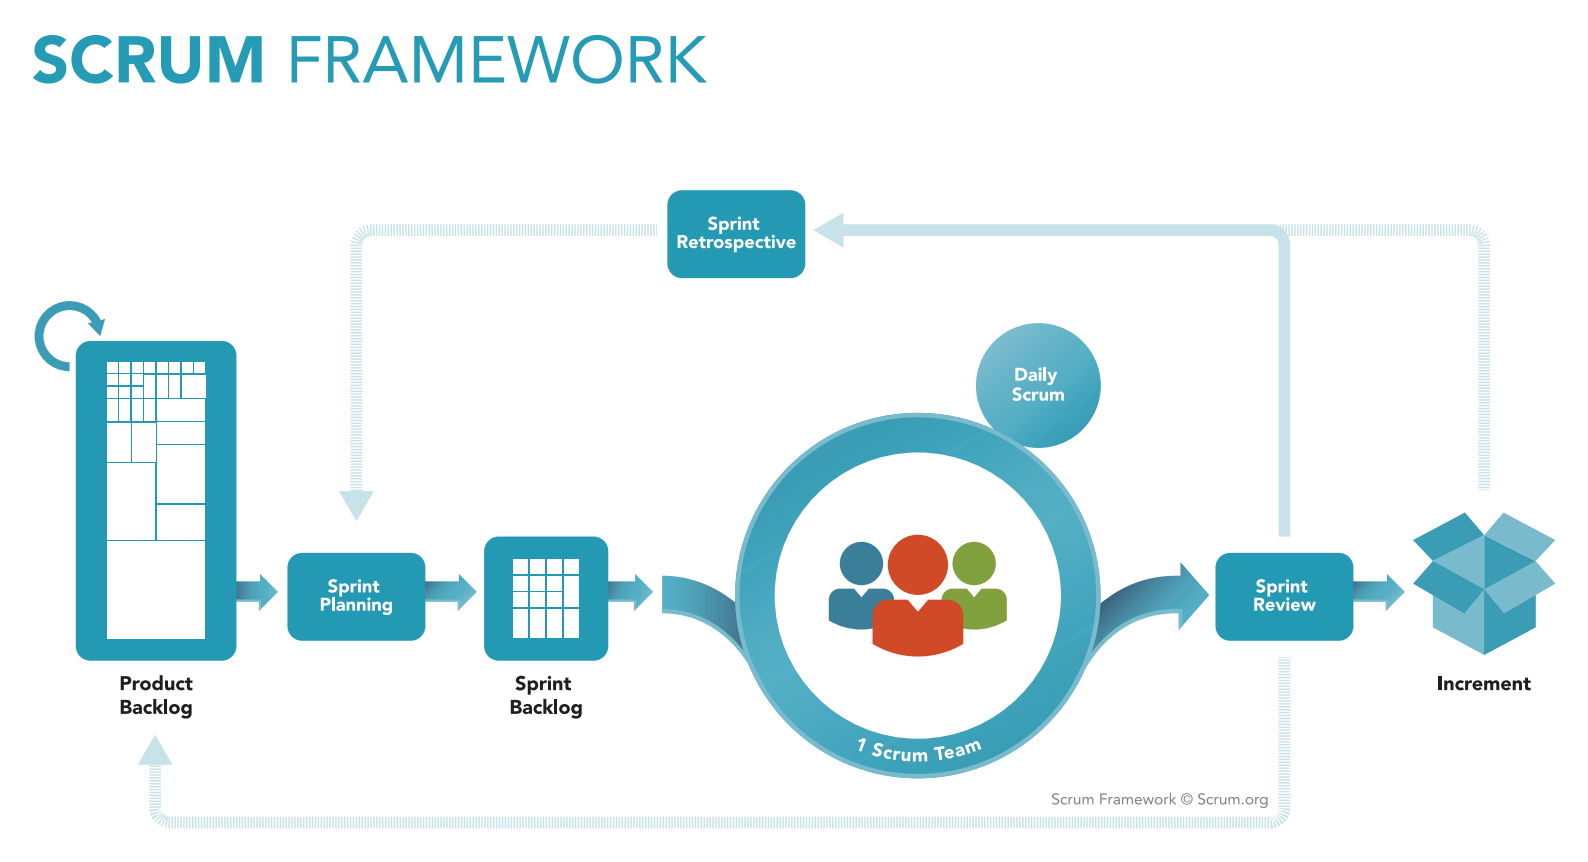
\includegraphics[width=15cm, keepaspectratio]{img/development/SCRUM}
  \caption{The scrum framework}
  \label{fig:scrum}
\end{figure}

\section{Iteration 0: Investigation and preliminary study} 
\label{sec:it0}
This is not an iteration itself, but it is a necessary part of the development, so we decided to include it as 'iteration 0' and here we will get the tools and the study we will need to make our plugin. 

At the beginning, there were a lot of things to explore. First of all, we have to study, understand and get used to Kibana and ElasticSearch, for that purpose, we will begin installing the actual version of Kibana and ElasticSearch (both version 4.0) using some no significant data to test it.

Later, we will build the development environment to create the plugin. We will study the plugin’s composition already existent in Kibana in order to gather the necessary information to build a new one, etc.

Once built the development environment, we will explore different visualization’s libraries of node’s networks to choose which fits best with the project. These are the libraries we will explore:

\begin{itemize}
\item Vis.js
\item Sigma.js
\end{itemize}

\subsection{Testing Kibana Client}

Before to start any software development, we have to learn the functioning and we have to get used to the tool the plugin will be developed for (Kibana, in this case). There’s no better way to learn than “explore” and “play” installing the latest version available (client version). From the official web page of Elastic, we will download the latest version available of Kibana (version 4) and the database ElasticSearch.  When these are downloaded and installed in the computer, we will initiate Kibana and, immediately, we will realize that we have to configure an “index pattern” (as it is explained in the subsection Kibana on chapter 2 - \ref{sec:kibana}). We can’t configure it yet, since there aren’t any data in ElasticSearch (because we have installed it from the ground), therefore, before configuring Kibana, we have to upload data to ElasticSearch.

To learn the management of Kibana and start “playing”, we don’t need significant data, so the best option is to download some “test data”. These can be found easily on internet; even the official web page of Elastic offers some of them. In our case, we will download some data that contains a set (~15.000) of public tweets, all collected on February, 5th 2015, between 12:00 and 12:05 (UTC+1) with index name “twitter”.

The next figure shows the configuration of the "twitter" index pattern:

\begin{figure}[H]
  \centering
  \includegraphics[width=15cm, keepaspectratio]{img/development/twitterindexpattern}
  \caption{Configuring index pattern}
  \label{fig:twitterindexpattern}
\end{figure}

Once the index pattern is configured, in the Discover tab we can see the chosen data of the time span, remembering it can be changed clicking on the top right page. In the list on the left, we will choose the fields we want to appear, clicking on them, and then the result shows up in a table with the fields chosen next to the time-field previously selected when we configured the index pattern. Above the table, we also notice a graphic that shows the data volume according to the chosen time-field.

\begin{figure}[H]
  \centering
  \includegraphics[width=15cm, keepaspectratio]{img/development/twitterdiscoverdata}
  \caption{Discover Data}
  \label{fig:twitterdiscoverdata}
\end{figure}


Now we have understood how the Discover tab works, we will build the first visualizations of these data. Inside “Visualize” we will choose amongst different kind of visualizations. These don’t have to be about the data, for example: the visualization “Markdown widget” consist of showing in format Markdown the inserted code in the left text area. We will build a visualization and we will save it with the “save” button.

\begin{figure}[H]
 \centering
  \subfloat[Markdown]{
    \includegraphics[width=0.50\textwidth]{img/development/twittermarkdown}}
  \subfloat[Pie chart]{
    \includegraphics[width=0.50\textwidth]{img/development/twitterpiechart}}
 \caption{Different examples of visualizations, with or without data}
 \label{f:fc2}
\end{figure}


When we have tested and saved some visualizations, we will see how the dashboard works to gather all these visualizations. In the "Dashboard" tab an empty dashboard will appear. Clicking “+”, we can add the saved visualizations. Once added, we can change their size, filter the data and move them into the dashboard, being the content completely active, iterative and responsive.

\begin{figure}[H]
  \centering
  \includegraphics[width=16cm, keepaspectratio]{img/development/twitterdashboard}
  \caption{Example of Dashboard}
  \label{fig:twitterdashboard}
\end{figure}


\subsection{Setting Up the Development Environment}

After getting used to Kibana and ElasticSearch, we will build a development environment of Kibana to observe the composition of the plugins of visualization to start creating plugins from the ground.

After getting used to Kibana and ElasticSearch, we will build a development environment of Kibana to observe the composition of the plugins of visualization to start creating plugins from the ground.

Following the documentation offered inside the repository of Kibana in the section corresponding to \textit{"CONTRIBUTING.md"}\footnote{\url{https://github.com/elastic/kibana/blob/master/CONTRIBUTING.md}}, we can build a development environment.

Searching about the Kibana’s code, we realize that the plugins (already existent) are developed inside separated folders in the directory \textit{"KIBANA\_HOME/src/core\_plugins/"}. We will study and come to the conclusion that the plugins have the next structure:

\begin{itemize}
\item \textbf{package.json}:  It is the regular npm package file, where it states the plugin’s information, such as the name, the version and the author. It also states the dependencies of JavaScript modules for its installation with the npm.
\item \textbf{index.js}: This is the main file, this code gets a reference to a kibana object passed to its module. The module must instantiate a new instance of a kibana plugin.

\begin{center}
\textit{NOTE: The code of this file is detailed in Appendix \ref{sec:indexjs}}
\end{center}

The uiExports object describe several extensions the plugin wants to add to the user interface. In this case, it use the visTypes array to register one visualization types. RequireJS will resolve plugins/plugin-name/ to the public folder of the plugin, where it can reference any file. 
 
\item \textbf{public/}: Folder where the plugin’s files are (of configuration, templates, controllers, etc.).
\item public/\textbf{plugin-name.js}: File where all the plugin’s information is recorded and defined (the files that compose it, if it uses the ElasticSearch data or not, etc.) It follows the next structure:

\begin{center}
\textit{NOTE: The code of this file is detailed in Appendix \ref{sec:pluginnamejs}}
\end{center}

The params object specify the template of the options that user can change and the defaults values.

For a visualization that uses data aggregation, Its need to specify exactly what aggregations the visualization needs or is allowed to have. These so called schemas will be added to the visualization description. To define schemas, it's necessary create a new Schemas object, which will take an array of objects in its constructor. Each object describes one aggregation it accept for the visualization. Each aggregation object have the following keys:

\begin{itemize}
\item \textbf{group}: either "metrics" or "buckets". Will define, which kind of aggregation it want to describe in this object.
\item \textbf{name}: the name (id) of this aggregation. It can use this later to get a reference to the different aggregations again.
\item \textbf{title}: the title shown to the user, when he adds the aggregation. Should describe how that aggregation will be visualized.
\item \textbf{min/max}: the number of minimum and maximum aggregations of that type, a user can add. E.g. the vertical bar chart has a bucket aggregation for "Split Bars". It is not limited (i.e. no max value specified) since it can split the bar as many times as the user wishes.
\item \textbf{aggFilter}: a filter on which aggregations should be allowed. It is an array of either aggregation types, that are allowed in this place (as shown in the metrics aggregation) or an array of aggregation types forbidden (each must be prefixed with a bang). In the later case all other aggregations are allowed. If the array has only one element you can also specify it as a string (as shown in the bucket aggregation). The types, that it can specify for metrics aggregations' aggFilter are the following: avg, cardinality, count, max, median, min, percentile\_ranks, percentiles, std\_dev, sum. The types, that it can specify for bucket aggregations' aggFilter are the following: date\_histogram, date\_range, filters, geohash\_grid, histogram, ip\_range, range, significant\_terms, terms.
\end{itemize}


\item public/\textbf{plugin-name.html}: Template of the plugin.
\item public/\textbf{plugin-name.less}: File that defines the plugin style.
\item public/\textbf{plugin-name\_controller.js}: File where all the plugin’s logic is programmed, the plugin’s controller. It follows the next format:

\begin{center}
\textit{NOTE: The code of this file is detailed in Appendix \ref{sec:pluginnamecontrollerjs}}
\end{center}

There are two variables inherited into the angular scope, that it will need. One is the vis variable, which holds information about your visualization and the settings the user chose. The other variable is named esResponse and holds the Elasticsearch response for the visualization. Kibana will automatically query Elasticsearch with the aggregations set by the user and taking into account currently set queries and filters.

To access the result of the aggregations we can look into "\$scope.esResponse.aggregations" (The object "resp" passed to the function corresponds to "\$scope.esResponse"). To find aggregations in that object we need their ids. To find the ids for a specific aggregation we can use several methods of "\$scope.vis.aggs" to find the id. For example:

\begin{lstlisting}[frame=single]
$scope.vis.aggs.bySchemaName['nameagg'][0].id
\end{lstlisting}

\item public/\textbf{plugin-name\_params.html}: File that defines some options of the visualization that will be shown when the user edits it. This is again a basic AngularJS HTML template. Inside the "vis" object (remember that is one of the two variables inherited into the angular scope) a key params exists. This should be used to store the parameters/options for the visualization. That’s why it binds the options to vis.params.*** (It would be more than one option).
\item public/\textbf{plugin-name\_params.js}: File where the logic of the options of the previous file is defined, it means, the controller of the plugin’s options. It follows this structure:

\begin{center}
\textit{NOTE: The code of this file is detailed in Appendix \ref{sec:pluginnameparamsjs}}
\end{center}

\end{itemize}

This is the structure we must follow when we create a new plugin.

\subsection{Choosing a Visualization Library}

At the same time of the study of the functioning of Kibana and its plugins, we have explored different kinds of data visualizations in form of social network to analyze them and choose which fits best to the project. Particularly, we have analyze the libraries VisJS\footnote{\url{http://visjs.org/index.html}} and SigmaJS\footnote{\url{http://sigmajs.org/}}. Both are under open source software license and they’re hosted publically in GitHub.

Sigma is a JavaScript library dedicated to graph drawing, these are a few simple examples that have been tested:

\begin{figure}[H]
 \centering
  \subfloat[]{
    \includegraphics[width=0.33\textwidth]{img/development/sigma1.png}}
  \subfloat[]{
    \includegraphics[width=0.33\textwidth]{img/development/sigma2.png}}
   \subfloat[]{
    \includegraphics[width=0.33\textwidth]{img/development/sigma3.png}}
 \caption{Examples of SigmaJS}
 \label{f:sigmaexamples}
\end{figure}

VisJS is a library that allows the data visualization in different ways, but we are interested in the social network. These are a few simple examples that have been tested:

\begin{figure}[H]
 \centering
  \subfloat[]{
    \includegraphics[width=0.33\textwidth]{img/development/visjs0.png}}
  \subfloat[]{
    \includegraphics[width=0.33\textwidth]{img/development/visjs1.png}}
   \subfloat[]{
    \includegraphics[width=0.33\textwidth]{img/development/visjs2.png}}
 \caption{Examples of VisJS}
 \label{f:sigmaexamples}
\end{figure}

For the project development, after the analysis of both libraries, we have agreed the use of VisJS. It has great advantages regarding SigmaJS; VisJS allows a biggest customizing of the node network, since it has a wider API. With it, we can improve the output of scalability when we have a big amount of data, change the network physics, handle many interaction events, the use of dynamic data, etc. Besides, VisJS has a very active community, improving and solving library mistakes every week.

\section{Iteration 1: First plugins}

The aim of this iteration is the plugins developments from the ground, starting from create a simple one and then a complex one, accessing to the data (schemas):

\begin{enumerate}
\item Develop a simple plugin without data.
\item Develop a complex plugin with data.
\end{enumerate}

\subsection{Plugin Without Data}

To start, the best option is the creation of a plugin in the simplest way possible, with no access to the data. The aim is the creation of a plugin that interprets a source code HTML added by the user and it shows it in the visualization area (similar to the plugin of visualization "Markdown"). 

We will name this plugin "prueba-vis" and we will proceed to program it following the structure of any plugin of Kibana (as we have already explained in the previous iteration).

\begin{lstlisting}[frame=single]
// package.json
{
  "name": "prueba_vis",
  "version": "1.0.0"
}
\end{lstlisting}

This is a test plugin, so we can continue just indicating the name and version of the plugin. In the main file "prueba-vis" we give information to the plugin.

The template of the plugin will be just the space Kibana leaves to visualize the plugin, so the template is just composed of a div that contains all that space. We see that the syntax is of Angular, as we will use controllers that will manage that space.

\begin{lstlisting}[frame=single]
<div ng-controller="KbnPruebaVisController" class="prueba-vis">
      <div ng-bind-html="html"></div>
</div>
\end{lstlisting}

It’s necessary that, in the left part of the visualization, the user has a text area so it can be inserted the HTML code that he/she wants to interpret. This text area is stated in the HTML file, where the params/options of the visualizations are defined (it means, in prueba-vis\_params.html):

\begin{lstlisting}[frame=single]
<div class="form-group">
  <label>Modifica aqui el html</label>
  <textarea ng-model="vis.params.html" class="form-control" rows="20"></textarea>
</div>
\end{lstlisting}

What the controller must do is to pick up the text entered by the user and, once interpreted, insert it in the div that we have indicated in the template. It is all made through elements and modules of AngularJS:

\begin{lstlisting}[frame=single]
$scope.$watch('vis.params.html', function (html) {
    if (!html) return;
    $scope.html = $sce.trustAsHtml(html);
});
\end{lstlisting}

As a result, in the screen of visualization we obtain a text area on the left, where the user inserts the HTML code. On the right, it will be where it will be shown the interpreted HTML code.

\begin{figure}[H]
  \centering
  \includegraphics[width=16cm, keepaspectratio]{img/development/html}
  \caption{Result of the visualization}
  \label{fig:pluginhtml}
\end{figure}


\subsection{Plugin With Data}

In this case, we want that the plugin shows a visualization of data aggregations. For that purpose, as we have already explained,we have to add an object “schemas” to the definition of the plugin, where there are specified the aggregations needed.

The idea is create a very simple tag cloud plugin, that shows the bucket name as a label and the result of the metrics aggregation determines the fontsize of the label. We need in total 2 aggregations, one for metric and the other for buckets:

\begin{lstlisting}[frame=single]
schemas: new Schemas([
	{
		group: 'metrics',
		name: 'tagsize',
		title: 'TagSize',
		min: 1,
		max: 1,
		aggFilter: ['count', 'avg', 'sum', 'min', 'max', 'cardinality', 'std_dev']
	},
	{
		group: 'buckets',
		name: 'tags',
		title: 'Tags'
		min: 1,
		max: 1,
	}
])
\end{lstlisting}

In the controller, to get into the chosen metric, the object \$scope.vis.aggs allows to Access to it through the attribute “name” we have given to the schema, in this case:

\begin{lstlisting}[frame=single]
	var metricsAgg = $scope.vis.aggs.bySchemaName['tagsize'][0];
\end{lstlisting}

And to access the buckets (where the data and aggregations are), first we have to obtain the id of the aggregation through the attribute “name”, given to the schema and after, inside the object “resp” (remembering this is the object where all the data of response are) we find the buckets with that id.

\begin{lstlisting}[frame=single]
	var tagsAggId = $scope.vis.aggs.bySchemaName['tags'][0].id;
	var buckets = resp.aggregations[tagsAggId].buckets;
\end{lstlisting}

Once obtained the buckets, to get the metric correspondent to each bucket, we have to iterate the buckets and pass each bucket to a function that has the object of the metrics obtained previously, giving as a result the value of the metric of that bucket.

\begin{lstlisting}[frame=single]
	$scope.tags = buckets.map(function(bucket) {
		var value = metricsAgg.getValue(bucket);
		return {
			label: bucket.key,
			value: value
		};
	});
\end{lstlisting}

Now we have all the data and we just have to represent it. As a result, choosing “Count” as metric and the field "author\_name" as bucket, we obtain the next visualization.

\begin{figure}[H]
  \centering
  \includegraphics[width=16cm, keepaspectratio]{img/development/tagcloud}
  \caption{Result of the TagCloud visualization}
  \label{fig:plugintagcolud}
\end{figure}

\section{Iteration 2: Integration}

Once we have learned how to create the plugins, the next step is to integrate the visualization library with Kibana for its later development with it. Therefore, the aims of this iteration are:

\begin{enumerate}
\item Integration of the library.
\item Beginning Develop a simple plugin using the library.
\end{enumerate}

\subsection{Integration of the library}

VisJS can be installed in many ways, adding the reference of its files js, installing with bower or as we are most interested in, installing it as an npm package. VisJS is in the list of available packages of npm; the ideal way for its installation is adding VisJS as a dependency in the file “package.json” of the plugin, this way:

\begin{lstlisting}[frame=single]
{
  "name": "network_vis",
  "version": "1.0.0",
  "authors": [
  "David Moreno Lumbreras <dmorenolumb@gmail.com>"
  ],
  "dependencies" : {
    "vis": "4.16.1"
  }
}
\end{lstlisting}

As we have already explained (in the npm subsection on chapter 2 - \ref{sec:nodejsnpm}), when the dependency is added, it is necessary execute the command “npm install” in the directory where the file package.json is, so npm automatically downloads and installs the module inside a folder named "node\_modules".

Once downloaded and installed the library, in order to use it where we want (in this case, the plugin controller) we must download the library through require (remembering that Kibana has RequireJS):

\begin{lstlisting}[frame=single]
	const visN = require('vis');
\end{lstlisting}

Inside the code, he API of the library will be available with the constant variable “visN”.

\subsection{Plugin using VisJS}

The main idea is to create a plugin from the ground and develop it and improve it step by step until the final product. The plugin will be called "Network Plugin" and, as we have already seen, it will follow the same structure of the Kibana plugins.

We create a plugin that shows just a simple node network using he library, which means, to integrate one of the basic examples of VisJS inside Kibana. The node network is drawn on a canvas that the library itself inserts in a div previously chosen; the div must be inside the template of the plugin, this way: 

\begin{lstlisting}[frame=single]
	<div ng-controller="KbnNetworkVisController" class="network-vis" id="mynetwork"</div>
\end{lstlisting}

We will initiate a node network in the controller through the identifier of the div and the test data inserted on the code:

\begin{lstlisting}[frame=single]
	var container = document.getElementById('mynetwork');
	var network = new visN.Network(container, data);
\end{lstlisting}

As a result we will obtain the next example:

\begin{figure}[H]
  \centering
  \includegraphics[width=16cm, keepaspectratio]{img/development/integration}
  \caption{Simple Plugin using VisJS}
  \label{fig:examplepluginvisjs}
\end{figure}


\section{Iteration 3: Visualization with ElasticSearh data}

In the middle of the development, Elastic published a new version of Kibana, the version 5. In favour of the plugin to be published and used always in its latest version available, it’s been decided to upgrade Kibana to the latest version and continuing with the development.

Once the simple plugin is created with the visualization library, we will upload and use the data that the product owner has given to us and we will add aggregations to show the visualization with these data of ElasticSearch. When the data network shows up, its insertion will be tested inside a dashboard to prove if it is responsive to the change of dynamic height and width next to other kind of visualizations. The aims of this iteration are these:

\begin{enumerate}
\item Migration to version 5.
\item Add Schemas to the plugin.
\item Build code for data visualization.
\item Dashboard Integration. 
\end{enumerate}

\subsection{Migration}

The step of migrate our plugin of Kibana 4 to Kibana 5 is simple, there are barely changes in the way of develop a plugin of visualization. The only one change to stand out is the way of import the files of the plugin with the main controller, since before it was done with RequireJS and in this version the files are imported with "import" of JavaScript.

\subsection{Adding Schemas}

The network will relate two fields to be chosen, so he aggregations will be two schemas of buckets, one for each field. As it only makes sense to show the fields of the database in form of nodes, we will restrict the choice of the kind of bucket to just “terms”. 

\begin{lstlisting}[frame=single]
{
   group: 'buckets',
   name: 'node',
   title: 'Node',
   min: 1,
   max: 2,
   aggFilter: ['terms']//Only have sense choose terms
},
\end{lstlisting}

\subsection{Building code}

When the data of the aggregations are obtained, we must parse them to the format required by the visualization library. All the code is programmed in JavaScript language, using modules of AngularJS and JQuery. Besides, it’s been written all the information of the plugin, adding its title, description and icon. We see in the list of the plugins how it appears:

\begin{figure}[H]
  \centering
  \includegraphics[width=10cm, keepaspectratio]{img/development/networkinformation}
  \caption{Information}
  \label{fig:networkinformation}
\end{figure}

With the code already parsed, we obtain a network like this:

\begin{figure}[H]
  \centering
  \includegraphics[width=16cm, keepaspectratio]{img/development/visualizationwithdata}
  \caption{Network with Data}
  \label{fig:visualizationwithdata}
\end{figure}

\subsection{Dashboard Integration}
\label{sec:dashboardintegration}

The visualization library VisJS hasn’t got implemented the dynamic change of height and width when the div where the network is drawn, changes. This is a big problem, since in the dashboard of Kibana, the user can change the size of each visualization anytime and the content must adapt to the new height and width.
To this problem, we have explored extern libraries that capture the launched CSS event when a div size is changed. One of the libraries that captures this event is the library ResizeSensor, that allows binding a div so when its CSS attributes are changed, it allows to do any other programmed task.

In this case, we have bound the div that contains the visualization to ResizeSensor, and when it captures the event of change of size, the network will be redrawn and it will adapt to its new size. VisJS allows to redraw the network in a given height and width with a function of its API. It works this way:

\begin{lstlisting}[frame=single]
          new ResizeSensor(viscontainer, function() {
              network.setSize('100%', viscontainer.clientHeight);
          });
\end{lstlisting}

In the next figures, we will see the final result of the network of different sizes:

\begin{figure}[H]
 \centering
  \subfloat[Small size]{
    \includegraphics[width=0.5\textwidth]{img/development/integrationdashboard1}}
  \subfloat[Big size]{
    \includegraphics[width=0.5\textwidth]{img/development/integrationdashboard2}}
 \caption{Network with differents sizes}
 \label{f:sigmaexamples}
\end{figure}



\section{Iteration 4: Different ways to represent and Optimization}

The next step is add the functionality so the network can be represented of different ways, in our case, we will add the option of represent a network relating two different kind of nodes (one per chosen field) and the option of represent the network with a kind of node and a relation between them with a field to choose.

Once these functionalities are created, we will optimize the code and the options of network representation so the loading time aren’t very high and the visualization is the as clear as possible.

\subsection{Changing Schemas and Building differents ways}

To give the user the chance to choose a kind of network or another, we must make a change in the schemas.

\begin{lstlisting}[frame=single]
{
        group: 'buckets',
        name: 'first',
        icon: 'fa fa-circle-thin',
        mustBeFirst: 'true',
        title: 'Node',
        min: 1,
        max: 2,
        aggFilter: ['terms']
      },
      {
        group: 'buckets',
        name: 'second',
        icon: 'fa fa-random',
        title: 'Relation',
        max: 1,
        aggFilter: ['terms']
      },
}
\end{lstlisting}

It has been added an aggregation of bucket type (Relation) that will be the one that allows choosing the field related to the chosen nodes in the previous aggregation. So if the user wants to show a network with an only kind of node and field that relates them, he/she will have to choose "Node" in the first bucket aggregation and "Relation" in the second one. Nevertheless, if the user wants to show a network with two kind of nodes related between them, he/she will have to choose "Node" in the first bucket aggregation and again "Node" in the second one.
 
\begin{figure}[H]
  \centering
  \includegraphics[width=6cm, keepaspectratio]{img/development/noderelation}
  \caption{Buckets available}
  \label{fig:noderelationbuckets}
\end{figure}

Inside the code the data is processed and parsed depending on the kind of network that has been chosen. This way, interpreting the data, the visualization library shows two kind of different network:

\begin{lstlisting}[frame=single]
if($scope.vis.aggs.bySchemaName['first'].length >= 1 && !$scope.vis.aggs.bySchemaName['second']){ //This is when we have 2 nodes}
	//Processing the data of the Node-Node network
}else if($scope.vis.aggs.bySchemaName['first'].length == 1 && $scope.vis.aggs.bySchemaName['second']){
	//Processing the data of the Node-Relation network
}
\end{lstlisting}

In the case of choose twice "Node" and "Relation" as aggregations, an error message will show up in the visualization space indicating the right way of the choice:

\begin{figure}[H]
  \centering
  \includegraphics[width=15cm, keepaspectratio]{img/development/errornoderelation}
  \caption{Error shows at incorrect selection}
  \label{fig:errornoderelation}
\end{figure}


\subsection{Optimization}

When the aggregations produce a big amount of data, the program must analyze and process them in an optimal and quick way in order to not interfere in the quality and experience of the user.

Inside the code, the data are processed in an optimal way, for example fulfilling some tasks inside the same loop, using functions of JavaScript instead of the use of JQuery, etc.

The visualization library suffers a delay in rendering the network when it has to process a big amount of nodes and edges, in order to relieve this user experience, a “Loading…” message has been added so the user knows that the visualization is loading and he/she doesn’t thinks something has gone wrong.
 
\begin{figure}[H]
  \centering
  \includegraphics[width=4cm, keepaspectratio]{img/development/loading}
  \caption{Loading network}
  \label{fig:errornoderelation}
\end{figure}

The same way, when the network has a lot of nodes and edges, a special option of the network is applied, that decreases and optimizes the distribution and physics of the nodes/edges in order to avoid that the browser slows down. Amongst these options, there is the option of hiding the edges when a node can be dragged; the gravitational constants are less strong, etc.

\section{Iteration 5: Customization}

The aim of this iteration is to add functionalities to the plugin so that the final user can modify the network and adapt it to the criteria he/she has. We will proceed to add different functionalities of customization, through aggregations and options. The aims of this iteration are these:

\begin{itemize}
\item Add aggregations for edge and node size and node color.
\item Add options changing params.
\end{itemize}

\subsection{Adding more aggregations}

The aggregations of metric type match perfectly to assign sizes to the nodes and edges of the network, since a result of the metric is always a numeric value.

\begin{lstlisting}[frame=single]
	  {
        group: 'metrics',
        name: 'size_node',
        title: 'Node Size',
        max: 1
      },
      {
        group: 'metrics',
        name: 'size_edge',
        title: 'Edge Size',
        max: 1,
      },
\end{lstlisting}

On the other hand, it may happen that a group of nodes have something in common (for example, that the nodes are people and these people belong to an organization) and it’s convenient gather them, drawing them in the same color. For this case, it will be added an aggregation of bucket type that allows choosing a field, each node will be drawn in a color depending on the chosen field.

\begin{lstlisting}[frame=single]
      {
        group: 'buckets',
        name: 'colornode',
        icon: 'fa fa-paint-brush',
        title: 'Node Color',
        max: 1,
        aggFilter: ['terms']
      }
\end{lstlisting}

This aggregation must be added the last one of the list of aggregations (below the "Node" or Relation) so that the answer that Kibana sends back consulting ElasticSearch has sense. It has been added an error message when the “Node Color” aggregation isn’t the last selected.
The chosen colors must be random and, at the time, mustn’t repeat either be similar amongst them. For it, it has been decided to use the module “RandomColor” (installed through npm), which API allows generating attractive colors to the sight and, through programmed logic in the controller, won’t be repeated the generated colors.

With these improvements, we will obtain a network with more information, like this:
 
\begin{figure}[H]
  \centering
  \includegraphics[width=16cm, keepaspectratio]{img/development/sizecolornetwork}
  \caption{Network with Size and Color}
  \label{fig:sizecolornetwork}
\end{figure}

\subsection{Adding options}

Besides, it has been added the option of changing the next parameters of the visualization:

\begin{itemize}
\item Background color and the default color of the nodes.
\item Min and Max size of the nodes/edges.
\item Shapes of the nodes.
\item Top values of the metrics, forcing the results of the metrics that are above this value.
\item The min value of "Node Size" metric; the nodes with a value below this, will not be shown.
\item Possibility of hide the labels of the nodes.
\item Possibility of show a Popup when the user hover a node.
\item Possibility of show a Legend with the used colors.
\end{itemize}

These changes have been added in the tab “Options” of the visualization, modifying the file that contains the template in HTML of the options/parameters of the plugin.

\begin{figure}[H]
 \centering
  \subfloat[1/2]{
    \includegraphics[width=4cm]{img/development/params1}}
  \subfloat[2/2]{
    \includegraphics[width=4cm]{img/development/params2}}
 \caption{Params of the Network}
 \label{f:paramsnetwork}
\end{figure}
 
%%%%%%%%%%%%%%%%%%%%%%%%%%%%%%%%%%%%%%%%%%%%%%%%%%%%%%%%%%%%%%%%%%%%%%%%%%%%%%%%
%%%%%%%%%%%%%%%%%%%%%%%%%%%%%%%%%%%%%%%%%%%%%%%%%%%%%%%%%%%%%%%%%%%%%%%%%%%%%%%%
% RESULTADOS %
%%%%%%%%%%%%%%%%%%%%%%%%%%%%%%%%%%%%%%%%%%%%%%%%%%%%%%%%%%%%%%%%%%%%%%%%%%%%%%%%
\cleardoublepage
\chapter{Design and results}
\label{chap:dai}

\section{Introduction}
\label{sec:dint}

In this chapter we will describe the aspects of the final plugin. We will start defining its structure, in code and in visualization. Then, we will explain its functioning next to a user's guide in order to define de different types of visualization that the plugin has. Finally, we will test the plugin with data offered by the product owner; besides, we will show the results obtained by extern people that have downloaded and installed our plugin. 

\section{Structure}


As we have already explained (in the iteration 0 on chapter 3 - \ref{sec:it0}), in order to develop a plugin for Kibana, the plugin must follow a predefined structure of files and folders where each specific code (controller, template, style) will be inside a file. This group of files and folders must be inside a folder with the name of the plugin, and this one must be inside the folder “plugin” of the home directory of Kibana. This way, when Kibana initiates it will recognize and add the plugin to the application. Therefore, our plugin follows the next structure: 

\begin{figure}[H]
  \centering
  \includegraphics[width=10cm, keepaspectratio]{img/results/codediagram2}
  \caption{Diagram of the files}
  \label{fig:codediagram}
\end{figure}

Each file codes are detailed in the Appendix \ref{sec:plugincode}. 

Following, we will explain the visual structure of the plugin, which means, how is its visualization page inside Kibana.

In the list of possible visualizations to choose, we will see the way our plugin appears (corresponding to the item framed in red). The information corresponds to a title, a little description and an icon of the pack of icons “font-awesome” already included in Kibana: 

\begin{figure}[H]
  \centering
  \includegraphics[width=16cm, keepaspectratio]{img/results/lista}
  \caption{Network plugin in visualization list}
  \label{fig:listpluginsresults}
\end{figure}


At the right of the list, we will see another list of visualizations saved, each one matches with a name and the icon of the type of visualization that corresponds.

When our plugin is selected to create a visualization (Network Plugin) it is shown the next page: 

\begin{figure}[H]
  \centering
  \includegraphics[width=16cm, keepaspectratio]{img/results/pagevis}
  \caption{Network plugin main page}
  \label{fig:pagevisnetwork}
\end{figure}

The blue frame corresponds to the area of visualization of the plugin; in  that area is where the resulting network will be drawn. The red frame indicates the election area of aggregations for the visualizations, since it is marked with the tab “Data” as it says the figure. There is the possibility of choosing some type of metrics and buckets, they are detailed he next way: 

\begin{itemize}
\item \textbf{Node/Edge Size}: It allows choosing a metric; the obtained value of that metric will indicate the size of the node/edge.
\item \textbf{Node}: It allows to choose a field that will define the nodes of the resulting network. The results can be ordered according to a Custom Metric or alphabetically (Terms), at the same time, it allows choosing a limited number of data and order them in an ascendant/descendant way. This type of bucket can be chosen twice in the case of wanting a network that relates two different nodes, one per chosen example.
\item \textbf{Relation}: This type of bucket can be only chosen if the bucket selected previously corresponds to one "Node" type; at the same time, there can only be one bucket of type of "Node". This bucket allows selecting field that will define the relation between the nodes. The results can be ordered according to a Custom Metric or alphabetically (Terms). At the same time, it allows choosing a limited number of data and order them in an ascendant/descendant way.
\item \textbf{Node Color}: This type of bucket is optional, this bucket will be bound to the color of the first bucket of "Node" type, which means, it will give the color to the chosen nodes of the first bucket "Node". This bucket must always be selected the last one in order to avoid errors. The results can be ordered according to a Custom Metric or alphabetically (Terms). At the same time, it allows choosing a limited number of data and order them in an ascendant/descendant way. 
\end{itemize}

\begin{figure}[H]
 \centering
  \subfloat[Metric displayed]{
    \includegraphics[width=4.5cm]{img/results/metric}}
  \subfloat[Bucket displayed]{
    \includegraphics[width=4.5cm]{img/results/bucket}}
 \caption{Example of "Node Size" metric and "Node" bucket displayed}
 \label{f:metricbucketdisplayed}
\end{figure}

When we select the tab “Options”, it appears a list of the options to customize the visualization. Each option has its function: 

\begin{itemize}
\item \textbf{Default colors}: It allows selecting the background color and the default color of the nodes.
\item \textbf{Size}: It has two values, a maximum and a minimum for the nodes and the edges; these values define the maximum and a minimum size that nodes and edges can have.
\item \textbf{Shapes}: It allows selecting from a list, the shape that the nodes have.
\item \textbf{Extra}: 
\begin{itemize}
\item \textbf{Show labels}: When this option is activated, the label of each node will appear. If it is deactivated, the nodes without texts will appear.
\item \textbf{Show Popup}: When this option is activated, a popup will appear when the mouse pass by the nodes; in the popup will appear the label of each node and, if the bucket “Node Color” is selected, it will also appear he label of that aggregation.
\item \textbf{Show Color Legend}: When this option is activated, it will show a legend drawn inside the canvas that will give information of the node colors. This will only make sense and will be visible when the bucket “Node Color” is selected. 
\end{itemize}
\item \textbf{Top values}: These values will define the maximum value possible that can be obtained of each chosen metric ("Node Size" and "Edge Size"), in such a way that if we obtain a value above what is indicated in this option, it will be forced to the introduced value.
\item \textbf{Don't show nodes below this value}: This value define the minimum value that "Node Size" metric can have, if the value of the "Node Size" metric of a node is below this value, the node will not be shown.
\end{itemize}

In the next figure, we can see the tab “Options” with its entire options, the shown values are the default ones:

\begin{figure}[H]
 \centering
  \subfloat[1/2]{
    \includegraphics[width=4cm]{img/development/params1}}
  \subfloat[2/2]{
    \includegraphics[width=4cm]{img/development/params2}}
 \caption{Options of the network}
 \label{f:optionsnetwork}
\end{figure}

\section{User Guide}

Later, we will define a user guide, explaining step by step how to produce each type of network visualization and how to show its functionality. There are many ways to create a network visualization, each one according to the criteria of the user and the type of network that he/she wants to obtain. Then, we will explain how to produce each type of network from the ground.

\subsection{Network with only nodes and no relation}

In order to create a network that contains only nodes not related between them, we have to follow the next steps:

\begin{enumerate}
\item Select "Node" aggregation in buckets.
\item Select the field that will define the nodes in the “Field” tab, establish how it is going to be the order and how many data you want to obtain in Size. \textit{Optional: you can assign it an specific label to this aggregation through the input "Custom Label".}
\item Click “Play” button in order to load the visualization.
\end{enumerate}

As a result, we obtain the next type of visualization:

\begin{figure}[H]
  \centering
  \includegraphics[width=16cm, keepaspectratio]{img/results/onlynodes}
  \caption{Example of only nodes network}
  \label{fig:onlynodes}
\end{figure}


\subsection{Network with one type of nodes}

In order to create a network that contains one type of node related between them, we have to follow the next steps:

\begin{enumerate}
\item Select "Node" aggregation in buckets.
\item Select the field that will define the nodes in the “Field” tab, establish how it is going to be the order and how many data you want to obtain in Size. \textit{Optional: you can assign it an specific label to this aggregation through the input "Custom Label". }
\item Select "Relation" aggregation in buckets.
\item Select the field that will define the node relation in the “Field” tab, establish how it is going to be the order and how many data you want to obtain in Size. \textit{Optional: you can assign it an specific label to this aggregation through the input "Custom Label". }
\item Click “Play” button in order to load the visualization.
\end{enumerate}

As a result, we obtain the next type of visualization:

\begin{figure}[H]
  \centering
  \includegraphics[width=16cm, keepaspectratio]{img/results/nodesrelated}
  \caption{Example of one type of nodes, related to each other}
  \label{fig:nodesrelated}
\end{figure}

\subsection{Network with two type of nodes}

In order to create a network that contains two type of nodes related between them, we have to follow the next steps:

\begin{enumerate}
\item Select "Node" aggregation in buckets.
\item Select the field that will define the first type of node in the “Field” tab, establish how it is going to be the order and how many data you want to obtain in Size. \textit{Optional: you can assign it an specific label to this aggregation through the input "Custom Label". }
\item Select "Node" aggregation in buckets.
\item Select the field that will define the second type of node in the “Field” tab, establish how it is going to be the order and how many data you want to obtain in Size. \textit{Optional: you can assign it an specific label to this aggregation through the input "Custom Label". }
\item Click “Play” button in order to load the visualization.
\end{enumerate}

If the two fields have something in common, the nodes that belong to each field will appear linked. As a result, the next type of visualization will be obtained:

\begin{figure}[H]
  \centering
  \includegraphics[width=16cm, keepaspectratio]{img/results/nodenode}
  \caption{Example of two type of related nodes}
  \label{fig:nodenode}
\end{figure}

\subsection{Add Node Color}

In order to add color to the nodes according to the chosen field, it is necessary to build one of the networks previously described and follow these steps:

\begin{enumerate}
\item Build a network of those ones previously described.
\item Select "Node" Color aggregation in buckets.
\item Select the field that will define the node color in the “Field” tab, establish how it is going to be the order and how many data you want to obtain in Size. \textit{Optional: you can assign it an specific label to this aggregation through the input "Custom Label". }
\item Click “Play” button in order to load the visualization.
\end{enumerate}

As a result, we obtain the next type of visualization:

\begin{figure}[H]
  \centering
  \includegraphics[width=16cm, keepaspectratio]{img/results/nodecolor}
  \caption{Example of colored nodes}
  \label{fig:nodecolor}
\end{figure}

\subsection{Types of Error on selecting buckets}

There are three type of possible errors building a network:

\begin{itemize}
\item The aggregations have been configured in order to the aggregation or aggregations “Node” must be selected the first ones compulsory; Otherwise, it will appear the next Warning message: 
 
\begin{figure}[H]
  \centering
  \includegraphics[width=6cm, keepaspectratio]{img/results/nodefirsterror}
  \caption{Warning message when "Node" is not the first selection}
  \label{fig:noderror}
\end{figure}

\item When it is chosen as aggregations, the aggregation “Node” twice and the aggregation “Relation”, it will be shown an error message in the visualization area:

\begin{figure}[H]
  \centering
  \includegraphics[width=16cm, keepaspectratio]{img/results/errornodenoderelation}
  \caption{Error when is selected "Relation" and 2 times "Node"}
  \label{fig:errornodenoderelation}
\end{figure}

\item So that the data obtained from the chosen aggregations make sense, the aggregation “Node Color” must be selected the last one, otherwise, it will be shown the next error message in the visualization area:
 
\begin{figure}[H]
  \centering
  \includegraphics[width=16cm, keepaspectratio]{img/results/errornodecolor}
  \caption{Error when "Node Color" is not the last selection}
  \label{fig:errornodecolor}
\end{figure}

\end{itemize}

\subsection{Add Node/Edge Size Customization}

In order to add sizes to the nodes and edges according to a metric, it is necessary to follow these steps:

\begin{enumerate}
\item Select "Node/Edge Size" aggregation in metrics.
\item Select a type of metric that will define the size of the node/edge, in case of selecting a type that needs a field to obtain it, select the field in the “Field” tab. \textit{Optional: you can assign it an specific label to this aggregation through the input "Custom Label".}
\item Click “Play” button in order to load the visualization.
\end{enumerate}

As a result, we obtain the next type of visualization:

\begin{figure}[H]
  \centering
  \includegraphics[width=16cm, keepaspectratio]{img/results/sizes}
  \caption{Example with "Node" and "Node Size" selected}
  \label{fig:sizes}
\end{figure}


\subsection{Change options}

In the “Options” tab, it can be changed and customize the different aspects of visualization, for example, change the background color, the node shape, add a color legend to the visualization, hide the node labels and show a Popup with the information of the node. First, we change the options according to what we like. Later, click “Play” button in order to load the visualization.

As a result, we obtain the next type of visualization:

\begin{figure}[H]
  \centering
  \includegraphics[width=16cm, keepaspectratio]{img/results/optionschanged}
  \caption{Example with Options changed}
  \label{fig:optionschanged}
\end{figure}

\subsection{Save and Integrate in a dashboard}

In order to show a visualization inside a dashboard, it is necessary to save it previously. Inside the page of the visualization, clicking the “Save” button, we can save the visualization; we will be asked a name and we will accept.

Once saved, it is only necessary to add it inside a dashboard, into the “Dashboard” page, we have to click the “Add” button and, in the list of saved visualizations, we choose the one we want.

As we already explained in the Iteration 3 of the 3rd chapter - \ref{sec:dashboardintegration}, the plugin visualization is completely responsive to the dynamic change of size. As a result, we will have, for example, this dashboard:

\begin{figure}[H]
  \centering
  \includegraphics[width=16cm, keepaspectratio]{img/results/dashboard}
  \caption{Example of Dashboard with Network Plugin}
  \label{fig:dashboard}
\end{figure}

\section{Software hosting and Testing}
\label{sec:softhostest}

All the carried out tests in the previous section one have been done with a group of data offered by the product owner; these data correspond to logs with information of commits of repositories; in this case, the time-field that we will define when we initiate the index in Kibana will be the date of the commit.
These data have been imported to ElasticSearch through the tool elasticdump, in its repository is the necessary information to understand its functioning \footnote{\url{https://github.com/taskrabbit/elasticsearch-dump}}.
Some network visualization has been obtained from these data, for example a network which nodes are authors and repositories and there are edges between them if the authors have contributed in the repositories. Another network could be the one formed by one type of nodes that would be the authors, and the edges between them if they have contributed in the same repository; at the same time, the nodes could be the repositories and these could have edges if they have an author in common that has contributed in both repositories.\\

As it was told in the Introduction \ref{sec:softavail}, the plugin is hosted on GitHub and it is prepared to be installed in any Kibana 5; inside the file “README.md” there are the installation/remove steps, there are also little examples. As the plugin is hosted in such a way that any user of Kibana can install it following the steps, the Elastic team has published my plugin in their page of known plugins, offering it visibility so the users of Kibana can use it.

After publishing it, many people have tested the plugin, they have opened GitHub Issues, and contacted me by email in order to inform me of the errors and possible solutions to fix them. All these have been bearded in mind for the final product, since the intervention of other people have helped to find and solve little errors faster.

Since it is unique and new and it represents social networks, we have received many positive opinions appreciating the contribution that this plugin makes. For instance, amongst all the people that have tested the plugin, we have these examples:

\begin{figure}[H]
 \centering
  \subfloat[]{
    \includegraphics[width=0.5\textwidth]{img/results/test1}}
  \subfloat[]{
    \includegraphics[width=0.5\textwidth]{img/results/test2}}
 \caption{Testing examples of differents developers}
 \label{f:testdevelopers}
\end{figure}

Interesting pages:

\begin{itemize}
\item Project page: \url{https://dlumbrer.github.io/kbn_network/}
\item GitHub Repository: \url{https://github.com/dlumbrer/kbn_network}
\item User Guide: \url{https://github.com/dlumbrer/kbn_network/blob/master/USER_GUIDE.md}
\item Kibana Known-Plugins page: \url{https://github.com/elastic/kibana/wiki/Known-Plugins}
\end{itemize}

%%%%%%%%%%%%%%%%%%%%%%%%%%%%%%%%%%%%%%%%%%%%%%%%%%%%%%%%%%%%%%%%%%%%%%%%%%%%%%%%
%%%%%%%%%%%%%%%%%%%%%%%%%%%%%%%%%%%%%%%%%%%%%%%%%%%%%%%%%%%%%%%%%%%%%%%%%%%%%%%%
% CONCLUSIONES %
%%%%%%%%%%%%%%%%%%%%%%%%%%%%%%%%%%%%%%%%%%%%%%%%%%%%%%%%%%%%%%%%%%%%%%%%%%%%%%%%

\cleardoublepage
\chapter{Conclusions}
\label{chap:conclusions}
The aim of this project was the integration of visualization systems of social networks in complex systems of data visualization and interaction. Watching the result of the project, we can say we have fulfilled the main aim successfully. Besides, all the sub-goals have also been fulfilled:

It has been created a plugin for Kibana that allows to visualize the data in a social network way. Also, different libraries of visualization have been studied and, after choosing the most appropriate, it has been integrated in Kibana with the aim of use it in a visualization. It has been studied and learned the complete use of the tools Kibana and ElasticSearch for the development of this plugin. Once created the plugin, the aspects of Kibana have been modified so that the resulting network visualization is the most flexible as possible for the user. At the same time, more options that allow the library to obtain a biggest customization have been added. The visualization can be added to a dashboard by showing a full compatibility with other visualizations and with the dynamic changes of size and data. It is necessary to outstand that the plugin code is optimized so that when there is a big amount of data, the visualization doesn’t suffer a long delay and it shows up as clear and organized as possible.\\

One of the things that I’ve put more effort in is in the research of information of Kibana and ElasticSearch. Kibana is fairly a new tool; it changes its version with a lot of frequency and the community is right in the expansion (in this case, I had to migrate from version 4 to version 5), that’s the reason that only exist few information about creating plugins, solving errors, configuration, etc. Furthermore, the little there is, it is out of date. In most of the cases, when problems appeared or I didn’t find the way to complete a task, I had to “make a living” to solve everything; with no doubt, it has been a great challenge. When I had a knowledge background about Kibana, modifying aspects of the plugin to add more functionalities hasn’t been overly difficult, but it doesn’t mean that it has been a piece of cake, either, since managing such an amount of data that processes quickly so the user doesn’t notice the delay, has been a complex task that has taken too long.  But every effort has its rewards. The Kibana community has given their approval to my plugin; it has had a relative success, obtaining daily a mean of 90 viewers and 10 clones, altogether the plugin has received over 5000 views and 450 clones. Apart from the viewers, some people have contacted me by email to fix problems that have appeared to them or just to give me feedback of the plugin (around 20 emails), as I already said in chapter 4, section \ref{sec:softhostest}.


\section{Application of lessons learned}
\label{sec:aplication}

To get this project to success, it has been necessary to apply the knowledge learned in the degree, a very important one, what we learned about JavaScript, HTML, CSS. Amongst that knowledge, there are included those acquired about JQuery, Web Programming, programming in development environments, with frameworks, etc. But, all through the degree, as well as the knowledge of programming language, we have been taught to explore different ways of fulfilling the works, such as exploring different JavaScript libraries in order to decide which fits the best to the requirements.
Subjects like “Desarrollo de Aplicaciones Telemáticas” or "Ingeniería de Sistemas de la Información" have taught and guide us in Web Programming, for example, use and explore different JavaScript libraries, use software framework, etc. Also, there are some subjects that have provide us with the necessary knowledge in programming, but more in the “server” side, these subjects are “Servicios y Aplicaciones Telematicas" and "Ingeniería de Sistemas Telematicos", in which we have learned all the necessary of object-oriented programming using Python and Java.


\section{Lessons learned}
\label{sec:ll}

During this project, I’ve grown and learned knowledge, amongst them:

\begin{itemize}
\item Improve the skill in JavaScript, CSS and HTML language, also in AngularJS.
\item Use of the open source tool of data visualization and dashboard Kibana, as well as to develop for this tool and to fit to its peculiarities.
\item Manage of the NoSQL ElasticSearch database.
\item I’ve learned how to communicate with unknown people that have tested my project and, in certain way, have helped to its improvement.
\item Use of \LaTeX by developing the degree thesis, an interesting document preparation system.
\item Improvement of my English.  I’ve never written such a long essay and, thanks to this, I’m better now with the language.
\end{itemize}

\section{Future work}
\label{sec:fw}

This project isn’t finished yet, since each day more and more people download and install it for its use. It’s because of it that there is always something to fix or improve. The support of this project is constant and, thanks to the people’s feedback, it encourages me to keep contributing. We’ve suggested the next improvements:

\begin{itemize}
\item Add more customization options to the network.
\item Add more levels of data representation.
\item Add more interactivity in the network, like filters, etc.
\item Add another visualization library so that the user can decide with what library wants to render.
\item General optimization in order to improve the performance.
\item Creation of other plugins.
\end{itemize}


%%%%%%%%%%%%%%%%%%%%%%%%%%%%%%%%%%%%%%%%%%%%%%%%%%%%%%%%%%%%%%%%%%%%%%%%%%%%%%%%
%%%%%%%%%%%%%%%%%%%%%%%%%%%%%%%%%%%%%%%%%%%%%%%%%%%%%%%%%%%%%%%%%%%%%%%%%%%%%%%%
% AP�NDICE(S) %
%%%%%%%%%%%%%%%%%%%%%%%%%%%%%%%%%%%%%%%%%%%%%%%%%%%%%%%%%%%%%%%%%%%%%%%%%%%%%%%%
\cleardoublepage
\appendix
\chapter{Appendix}
\label{sec:appendix}
\section{Code template to create a plugin}

\subsection{index.js}
\label{sec:indexjs}

\begin{lstlisting}[frame=single]
module.exports = function(kibana) {
  return new kibana.Plugin({
    uiExports: {
      visTypes: [
        'plugins/plugin-name/plugin-name'
      ]
    }
  });
};
\end{lstlisting}

\subsection{plugin-name.js}
\label{sec:pluginnamejs}

\begin{lstlisting}[frame=single]
// Import of all plugin files 
import 'plugins/plugin-name/plugin-name.less';
import 'plugins/plugin-name/plugin-name_controller';
import 'plugins/plugin-name/plugin-name_params';

// Import VisSchemas and TemplatesVisTemplates of Kibana
import TemplateVisTypeTemplateVisTypeProvider from 'ui/template_vis_type/template_vis_type';
import VisSchemasProvider from 'ui/vis/schemas';

// Import the template of the visualization
import pluginNameTemplate from 'plugins/plugin-name/plugin-name.html'; 
 
function PluginNameProvider(Private) {
  var TemplateVisType = Private(TemplateVisTypeTemplateVisTypeProvider);
  
  // Include the Schemas class, which will be used to define schemas
  var Schemas = Private(VisSchemasProvider);

  return new TemplateVisType({
    name: 'pluginname', // The internal id of the visualization (must be unique)
    title: 'Plugin Title', // The title of the visualization, shown to the user
    description: 'This is a visualization', // The description of this vis
    icon: 'fa-xxx', // The font awesome icon of this visualization
    template: pluginNameTemplate,
    params: {
      defaults: {**},
      editor: '<plugin-name-params></plugin-name-params>'
    },
    schemas: new Schemas([
      {
        group: 'metrics',
        name: 'xxx',
        title: 'Xxx',
        min: 1,
        max: 1,
        aggFilter: ['count', 'avg', 'sum', 'min', 'max', 'cardinality', 'std_dev']
      },
      {
        group: 'buckets',
        name: 'yyy',
        title: 'Yyy',
        min: 1,
        max: 1,
        aggFilter: '!geohash_grid'
      },
      ...
    ])
  });
}

require('ui/registry/vis_types').register(PluginNameProvider);
\end{lstlisting}

\subsection{plugin-name\_controller.js}
\label{sec:pluginnamecontrollerjs}

\begin{lstlisting}[frame=single]
define(function (require) {
  // get the kibana/plugin-name module, and make sure that it requires the "kibana" module if it
  const module = require('ui/modules').get('kibana/plugin-name', ['kibana']);

  // add a controller to the module
  module.controller('PluginController', function ($scope, $sce, Private) {
    //Logic here
    $scope.$watch('esResponse', function(resp) {
    //Code
    }
  });

});
\end{lstlisting}

\subsection{plugin-name\_params.js}
\label{sec:pluginnameparamsjs}

\begin{lstlisting}[frame=single]
define(function (require) {
  const _ = require('lodash');

  require('ui/modules').get('kibana/plugin-name')
  .directive('pluginNameParams', function () {
    return {
      restrict: 'E',
      template: require('plugins/plugin-name/plugin-name_params.html'),
      link: function ($scope) {
        //Logic here
      }
    };
  });
});
\end{lstlisting}

\section{Plugin Code}
\label{sec:plugincode}

\subsection{index.js}

 \begin{lstlisting}[frame=single]
module.exports = function (kibana) {

  return new kibana.Plugin({
    uiExports: {
      visTypes: [
        'plugins/network_vis/network_vis'
      ]
    }
  });

};
\end{lstlisting}

\subsection{package.json}

 \begin{lstlisting}[frame=single]
{
  "name": "network_vis",
  "version": "5.0.0-rc1",
  "authors": [
  "David Moreno Lumbreras <dmorenolumb@gmail.com>"
  ],
  "dependencies" : {
    "vis": "4.16.1",
    "randomcolor": "0.4.4",
    "css-element-queries": "0.3.2"
  }
}
\end{lstlisting}

\subsection{network\_vis.html}

 \begin{lstlisting}[frame=single]
<div id="errorHtml"></div>
<div ng-controller="KbnNetworkVisController" class="network-vis" id="mynetwork" ng-style="{'background-color':vis.params.canvasBackgroundColor}">
</div>
<div id="loading" ng-style="{'background-color':vis.params.canvasBackgroundColor}">
  <div class="loading_msg">
    <p><strong>Loading network...</strong><i class="fa fa-clock-o" aria-hidden="true"></i></p>
  </div>
</div>
\end{lstlisting}

\subsection{network\_vis.js}

 \begin{lstlisting}[frame=single]
import "plugins/network_vis/network_vis.less";
import 'plugins/network_vis/network_vis_controller';
import TemplateVisTypeTemplateVisTypeProvider from 'ui/template_vis_type/template_vis_type';
import VisSchemasProvider from 'ui/vis/schemas';
import networkVisTemplate from 'plugins/network_vis/network_vis.html';
import networkVisParamsTemplate from 'plugins/network_vis/network_vis_params.html';

// register the provider with the visTypes registry
require('ui/registry/vis_types').register(NetworkVisTypeProvider);

// define the TableVisType
function NetworkVisTypeProvider(Private) {
  const TemplateVisType = Private(TemplateVisTypeTemplateVisTypeProvider);
  const Schemas = Private(VisSchemasProvider);

  // return the visType object, which kibana will use to display and configure new
  // Vis object of this type.
  return new TemplateVisType({
    name: 'network',
    title: 'Network',
    icon: 'fa-cogs',
    description: 'Displays a network node that link two fields that have been selected.',
    template: networkVisTemplate,
    params: {
      defaults: {
        showLabels: true,
        showPopup: false,
        showColorLegend: true,
        firstNodeColor: '#FD7BC4',
        secondNodeColor: '#00d1ff',
        canvasBackgroundColor: '#FFFFFF',
        shapeFirstNode: 'dot',
        shapeSecondNode: 'box',
        maxCutMetricSizeNode: 5000,
        maxCutMetricSizeEdge: 5000,
        minCutMetricSizeNode: 0,	
        maxNodeSize: 80,
        minNodeSize: 8,
        maxEdgeSize: 20,
        minEdgeSize: 0.1
      },
      editor: 'networkVisParamsTemplate'
    },

    hierarchicalData: function (vis) {
      return true;
    },

    schemas: new Schemas([
      {
        group: 'metrics',
        name: 'size_node',
        title: 'Node Size',
        max: 1
      },
      {
        group: 'metrics',
        name: 'size_edge',
        title: 'Edge Size',
        max: 1,
      },
      {
        group: 'buckets',
        name: 'first',
        icon: 'fa fa-circle-thin',
        mustBeFirst: 'true',
        title: 'Node',
        min: 1,
        max: 2,
        aggFilter: ['terms']//Only have sense choose terms
      },
      {
        group: 'buckets',
        name: 'second',
        icon: 'fa fa-random',
        title: 'Relation',
        max: 1,
        aggFilter: ['terms']
      },
      {
        group: 'buckets',
        name: 'colornode',
        icon: 'fa fa-paint-brush',
        title: 'Node Color',
        max: 1,
        aggFilter: ['terms']
      }
    ])
  });
}

export default NetworkVisTypeProvider;
\end{lstlisting}


\subsection{network\_vis.less}

\begin{lstlisting}[frame=single]
.network-vis{
  width: 100%;
  height: 100%;
}

div.vis-network-tooltip {
  position: absolute;
  visibility: hidden;
  padding: 5px;
  white-space: nowrap;

  font-family: verdana;
  font-size:14px;
  color:#000000;
  background-color: #f5f4ed;

  -moz-border-radius: 3px;
  -webkit-border-radius: 3px;
  border-radius: 3px;
  border: 1px solid #808074;

  box-shadow: 3px 3px 10px rgba(0, 0, 0, 0.2);
  pointer-events: none;
}

#errorHtml h1{
  color: white;
  text-align: center;
  background-color: red;
}

.loading_msg {
  height: 50px;
  width: 150px;
  border-radius: 10px 10px 10px 10px;
  border: 4px solid #FD7BC4;
  background-color: #00d1ff;
  text-align: center;
  line-height: 40px;
}
\end{lstlisting}


\subsection{network\_vis\_controller.js}

\begin{lstlisting}[frame=single]
define(function (require) {
  // get the kibana/table_vis module, and make sure that it requires the "kibana" module if it
  // didn't already
  const module = require('ui/modules').get('kibana/network_vis', ['kibana']);

  //import the npm modules
  const visN = require('vis');
  const randomColor = require('randomcolor');
  const ElementQueries = require('css-element-queries/src/ElementQueries');
  const ResizeSensor = require('css-element-queries/src/ResizeSensor');


  // add a controller to tha module, which will transform the esResponse into a
  // tabular format that we can pass to the table directive
  module.controller('KbnNetworkVisController', function ($scope, $sce, Private) {

    $scope.errorNodeColor = function(){
      $("#mynetwork").hide();
      $("#loading").hide();
      $("#errorHtml").html("<h1><strong>ERROR</strong>: Node Color must be the LAST selection</h1>");
      $("#errorHtml").show();

    }

    $scope.errorNodeNodeRelation = function(){
      $("#mynetwork").hide();
      $("#loading").hide();
      $("#errorHtml").html("<h1><strong>ERROR</strong>: You can only choose Node-Node or Node-Relation</h1>");
      $("#errorHtml").show();
    }

    $scope.initialShows = function(){
      $("#mynetwork").show();
      $("#loading").show();
      $("#errorHtml").hide();
    }

    $scope.startDynamicResize = function(network){
      for (i = 0; i < $(".vis-container" ).length; i++) {
         if($(".vis-container")[i].children[0].children[1] && $(".vis-container")[i].children[0].children[1].id == "mynetwork"){
           var viscontainer = $(".vis-container")[i];
           break;
         }
      };
      new ResizeSensor(viscontainer, function() {
          network.setSize('100%', viscontainer.clientHeight);
      });
    }

    $scope.drawColorLegend = function(usedColors, colorDicc){
       var canvas = document.getElementsByTagName("canvas")[0];
       var context = canvas.getContext("2d");

       context.fillStyle="#FFE8D6";
       var totalheight = usedColors.length * 25
       context.fillRect(canvas.width*(-2)-10, canvas.height*(-2)-18, 350, totalheight);

       context.fillStyle = "black";
       context.font = "bold 30px Arial";
       context.textAlign = "start";
       context.fillText("LEGEND OF COLORS:", canvas.width*(-2), canvas.height*(-2));

       var p=canvas.height*(-2) + 40;
       for(var key in colorDicc){
         context.fillStyle = colorDicc[key];
         context.font = "bold 20px Arial";
         context.fillText(key, canvas.width*(-2), p);
         p = p +22;
       }
    }


   $scope.$watchMulti(['esResponse', 'vis.params'], function ([resp]) {
      if (resp) {
        $("#loading").hide();
        if($scope.vis.aggs.bySchemaName['first'].length >= 1 && !$scope.vis.aggs.bySchemaName['second']){ //This is when we have 2 nodes
            $scope.initialShows();
            $(".secondNode").show();
            // Retrieve the id of the configured tags aggregation
            var firstFieldAggId = $scope.vis.aggs.bySchemaName['first'][0].id;
            if($scope.vis.aggs.bySchemaName['first'].length > 1){
              var secondFieldAggId = $scope.vis.aggs.bySchemaName['first'][1].id;
            }

            if($scope.vis.aggs.bySchemaName['colornode']){
              var colorNodeAggId = $scope.vis.aggs.bySchemaName['colornode'][0].id;
              var colorNodeAggName = $scope.vis.aggs.bySchemaName['colornode'][0].params.field.displayName;
              var colorDicc = {};
              var usedColors = [];
            }

            //Names of the terms that have been selected
            var firstFieldAggName = $scope.vis.aggs.bySchemaName['first'][0].params.field.displayName;
            if($scope.vis.aggs.bySchemaName['first'].length > 1){
              var secondFieldAggName = $scope.vis.aggs.bySchemaName['first'][1].params.field.displayName;
            }

            // Retrieve the metrics aggregation configured
            if($scope.vis.aggs.bySchemaName['size_node']){
              var metricsAgg_sizeNode = $scope.vis.aggs.bySchemaName['size_node'][0];
            }
            if($scope.vis.aggs.bySchemaName['size_edge']){
              var metricsAgg_sizeEdge = $scope.vis.aggs.bySchemaName['size_edge'][0];
            }

            // Get the buckets of that aggregation
            var buckets = resp.aggregations[firstFieldAggId].buckets;

            //////////////////////////////////////////////////DATA PARSED AND BULDING NODES//////////////////////////////////////////////////////////
            var dataParsed = [];
            // Iterate the buckets
            var i = 0;
            var dataNodes = buckets.map(function(bucket) {

              dataParsed[i] = {};
              dataParsed[i].keyFirstNode = bucket.key;


              //Metrics are for the sizes
              if(metricsAgg_sizeNode){
                // Use the getValue function of the aggregation to get the value of a bucket
                var value = metricsAgg_sizeNode.getValue(bucket);
                var sizeVal = Math.min($scope.vis.params.maxCutMetricSizeNode, value);

                //No show nodes under the value
                if($scope.vis.params.minCutMetricSizeNode > value){
                  dataParsed.splice(i, 1);
                  return;
                }
              }else{
                var sizeVal = 20;
              }

              dataParsed[i].valorSizeNode = sizeVal;
              dataParsed[i].nodeColorValue = "default";
              dataParsed[i].nodeColorKey = "default";


              //Iterate subbucket and choose the edge size
              if($scope.vis.aggs.bySchemaName['first'].length > 1){
                dataParsed[i].relationWithSecondNode = bucket[secondFieldAggId].buckets.map(function(buck) {
                  if(metricsAgg_sizeEdge){
                    var value_sizeEdge = metricsAgg_sizeEdge.getValue(buck);
                    var sizeEdgeVal = Math.min($scope.vis.params.maxCutMetricSizeEdge, value_sizeEdge);
                  }else{
                    var sizeEdgeVal = 0.1;
                  }

                  //Get the color of the node, save in the diccionary
                  if(colorNodeAggId && buck[colorNodeAggId].buckets.length > 0){
                    if(colorDicc[buck[colorNodeAggId].buckets[0].key]){
                      dataParsed[i].nodeColorKey = buck[colorNodeAggId].buckets[0].key;
                      dataParsed[i].nodeColorValue = colorDicc[buck[colorNodeAggId].buckets[0].key];
                    }else{
                      //repeat to find a NO-REPEATED color
                      while(true){
                        var confirmColor = randomColor();
                        if(usedColors.indexOf(confirmColor) == -1){
                          colorDicc[buck[colorNodeAggId].buckets[0].key] = confirmColor;
                          dataParsed[i].nodeColorKey = buck[colorNodeAggId].buckets[0].key;
                          dataParsed[i].nodeColorValue = colorDicc[buck[colorNodeAggId].buckets[0].key];
                          usedColors.push(confirmColor);
                          break;
                        }
                      }

                    }
                  }

                  return {
                    keySecondNode: buck.key,
                    countMetric: buck.doc_count,
                    widthOfEdge: sizeEdgeVal
                  };
                });
              }

              //assing color and the content of the popup
              var inPopup = "<p>" + bucket.key + "</p>"
              if(dataParsed[i].nodeColorValue != "default"){
                var colorNodeFinal = dataParsed[i].nodeColorValue;
                inPopup += "<p>" + dataParsed[i].nodeColorKey + "</p>";
              }else{
                var colorNodeFinal = $scope.vis.params.firstNodeColor;
              }

              i++;
              //Return the node totally builded
              var nodeReturn = {
                id: i,
                key: bucket.key,
                color: colorNodeFinal,
                shape: $scope.vis.params.shapeFirstNode,
                //size: sizeVal
                value: sizeVal
              }

              //If activated, show the labels
              if($scope.vis.params.showLabels){
                nodeReturn.label = bucket.key;
              }

              //If activated, show the popups
              if($scope.vis.params.showPopup){
                nodeReturn.title = inPopup;
              }

              return nodeReturn;
            });
            ////////////////////////////////////////////////////////////////////////////////////////////////////////////

            //////////////////////////////////////////////////BULDING EDGES//////////////////////////////////////////////////////////
            //Clean "undefinded" in the array
            dataNodes = dataNodes.filter(Boolean);
            var dataEdges = [];
            for(var n = 0; n<dataParsed.length; n++){
              //Find in the array the node with the keyFirstNode
              var result = $.grep(dataNodes, function(e){ return e.key == dataParsed[n].keyFirstNode;   });
              if (result.length == 0) {
                console.log("Error: Node not finded");
              } else if (result.length == 1) {
                //Finded the node, access to its id
                if($scope.vis.aggs.bySchemaName['first'].length > 1){
                  for(var r = 0; r<dataParsed[n].relationWithSecondNode.length; r++){
                    //Find in the relations the second node to relate
                    var nodeOfSecondType = $.grep(dataNodes, function(e){ return e.key == dataParsed[n].relationWithSecondNode[r].keySecondNode;   });
                    if (nodeOfSecondType.length == 0) {
                      //Not finded, added to the DataNodes - node of type 2
                      i++;
                      var newNode = {
                        id : i,
                        key: dataParsed[n].relationWithSecondNode[r].keySecondNode,
                        label : dataParsed[n].relationWithSecondNode[r].keySecondNode,
                        color: $scope.vis.params.secondNodeColor,
                        shape: $scope.vis.params.shapeSecondNode
                      };
                      //Add new node
                      dataNodes.push(newNode);
                      //And create the relation (edge)
                      var edge = {
                        from : result[0].id,
                        to : dataNodes[dataNodes.length-1].id,
                        value: dataParsed[n].relationWithSecondNode[r].widthOfEdge
                      }
                      dataEdges.push(edge);

                    } else if (nodeOfSecondType.length == 1) {
                      //Exist the node, create only the edge
                      var enlace = {
                        from : result[0].id,
                        to : nodeOfSecondType[0].id,
                        value: dataParsed[n].relationWithSecondNode[r].widthOfEdge
                      }
                      dataEdges.push(enlace);
                    } else {
                      console.log("Error: Multiples nodes with same id finded");
                    }
                  }
                }
              } else {
                console.log("Error: Multiples nodes with same id finded");
              }
            }
            ////////////////////////////////////////////////////////////////////////////////////////////////////////////


            ////////////////////////////////////Creation the network with the library//////////////////////////////////
            var nodesDataSet = new visN.DataSet(dataNodes);
            var edgesDataSet = new visN.DataSet(dataEdges);

            var container = document.getElementById('mynetwork');
            container.style.height = container.getBoundingClientRect().height;
            container.height = container.getBoundingClientRect().height;
            var data = {
              nodes: nodesDataSet,
              edges: edgesDataSet
            };
            //If it is too much edges, chnage the options to better optimization
            var options = {height: container.getBoundingClientRect().height.toString()};
            if(dataEdges.length > 200){
              var options = {
                height: container.getBoundingClientRect().height.toString(),
                physics:{
                  barnesHut:{
                    gravitationalConstant: -35000,
                    springConstant:0.01
                  }
                },
                "edges": {
                  "smooth": {
                    "forceDirection": "none",
                    "type": "continuous"
                  },
                  scaling:{
                    min:$scope.vis.params.minEdgeSize,
                    max:$scope.vis.params.maxEdgeSize
                  }
                },
                nodes: {
                  scaling:{
                    min:$scope.vis.params.minNodeSize,
                    max:$scope.vis.params.maxNodeSize
                  }
                },
                layout: {
                  improvedLayout: false
                },
                interaction: {
                  hover: true
                }
              };
            }
            console.log("Create network now");
            var network = new visN.Network(container, data, options);

            ////////////////////////////////////////////////////////////////////////////////////////////////////////////

            $scope.startDynamicResize(network);

            network.on("afterDrawing", function (canvasP) {
              $("#loading").hide();
              /// Draw the color legend if Node Color is activated
              if($scope.vis.aggs.bySchemaName['colornode'] && $scope.vis.params.showColorLegend){
                $scope.drawColorLegend(usedColors, colorDicc);
              }
            });

        }else if($scope.vis.aggs.bySchemaName['first'].length == 1 && $scope.vis.aggs.bySchemaName['second']){ //Node-Relation
          $scope.initialShows();
          $(".secondNode").hide();
           // Retrieve the id of the configured tags aggregation
          var firstFieldAggId = $scope.vis.aggs.bySchemaName['first'][0].id;
          var secondFieldAggId = $scope.vis.aggs.bySchemaName['second'][0].id;

          if($scope.vis.aggs.bySchemaName['colornode']){
            var colorNodeAggId = $scope.vis.aggs.bySchemaName['colornode'][0].id;
            var colorNodeAggName = $scope.vis.aggs.bySchemaName['colornode'][0].params.field.displayName;
            var colorDicc = {};
            var usedColors = [];

            //Check if "Node Color" is the last selection
            if($scope.vis.aggs.indexOf($scope.vis.aggs.bySchemaName['colornode'][0]) <= $scope.vis.aggs.indexOf($scope.vis.aggs.bySchemaName['second'][0])){
              $scope.errorNodeColor();
              return;
            }
          }

          //Names of the terms that have been selected
          var firstFieldAggName = $scope.vis.aggs.bySchemaName['first'][0].params.field.displayName;
          var secondFieldAggName = $scope.vis.aggs.bySchemaName['second'][0].params.field.displayName;

          // Retrieve the metrics aggregation configured
          if($scope.vis.aggs.bySchemaName['size_node']){
            var metricsAgg_sizeNode = $scope.vis.aggs.bySchemaName['size_node'][0];
          }
          if($scope.vis.aggs.bySchemaName['size_edge']){
            var metricsAgg_sizeEdge = $scope.vis.aggs.bySchemaName['size_edge'][0];
          }

          // Get the buckets of that aggregation
          if(resp.aggregations[firstFieldAggId]){
            var buckets = resp.aggregations[firstFieldAggId].buckets;
          }else{
            var buckets = resp.aggregations[secondFieldAggId].buckets;
          }

          //////////////////////////////////////////////////DATA PARSED AND BULDING NODES//////////////////////////////////////////////////////////
          var dataParsed = [];
          // Iterate the buckets
          var i = 0;
          var dataNodes = buckets.map(function(bucket) {

            dataParsed[i] = {};
            dataParsed[i].keyNode = bucket.key;

            //Metrics are for the sizes
            if(metricsAgg_sizeNode){
              // Use the getValue function of the aggregation to get the value of a bucket
              var value = metricsAgg_sizeNode.getValue(bucket);
              var sizeVal = Math.min($scope.vis.params.maxCutMetricSizeNode, value);

              //No show nodes under the value
              if($scope.vis.params.minCutMetricSizeNode > value){
                dataParsed.splice(i, 1);
                return;
              }
            }else{
              var sizeVal = 20;
            }

            dataParsed[i].valorSizeNode = sizeVal;
            dataParsed[i].nodeColorValue = "default";
            dataParsed[i].nodeColorKey = "default";


            //It depends of the priority of the selection to obtain the buckets
            if(bucket[secondFieldAggId]){
              var orderId = secondFieldAggId;
            }else{
              var orderId = firstFieldAggId;
            }

            dataParsed[i].relationWithSecondField = bucket[orderId].buckets.map(function(buck) {
              if(metricsAgg_sizeEdge){
                var value_sizeEdge = metricsAgg_sizeEdge.getValue(buck);
                var sizeEdgeVal = Math.min($scope.vis.params.maxCutMetricSizeEdge, value_sizeEdge);
              }else{
                var sizeEdgeVal = 0.1;
              }

              //Get the color of the node, save in the diccionary
              if(colorNodeAggId && buck[colorNodeAggId].buckets.length > 0){
                if(colorDicc[buck[colorNodeAggId].buckets[0].key]){
                  dataParsed[i].nodeColorKey = buck[colorNodeAggId].buckets[0].key;
                  dataParsed[i].nodeColorValue = colorDicc[buck[colorNodeAggId].buckets[0].key];
                }else{
                  while(true){
                    var confirmColor = randomColor();
                    if(usedColors.indexOf(confirmColor) == -1){
                      colorDicc[buck[colorNodeAggId].buckets[0].key] = confirmColor;
                      dataParsed[i].nodeColorValue = colorDicc[buck[colorNodeAggId].buckets[0].key];
                      usedColors.push(confirmColor);
                      break;
                    }
                  }

                }
              }

              return {
                keyRelation: buck.key,
                countMetric: buck.doc_count,
                widthOfEdge: sizeEdgeVal
              };
            });

            var inPopup = "<p>" + bucket.key + "</p>"
            if(dataParsed[i].nodeColorValue != "default"){
              var colorNodeFinal = dataParsed[i].nodeColorValue;
              inPopup += "<p>" + dataParsed[i].nodeColorKey + "</p>";
            }else{
              var colorNodeFinal = $scope.vis.params.firstNodeColor;
            }

            i++;
            //Return the node totally builded
            var nodeReturn = {
              id: i,
              key: bucket.key,
              color: colorNodeFinal,
              shape: $scope.vis.params.shapeFirstNode,
              //size: sizeVal
              value: sizeVal
            }

            //If activated, show the labels
            if($scope.vis.params.showLabels){
              nodeReturn.label = bucket.key;
            }

            //If activated, show the popus
            if($scope.vis.params.showPopup){
              nodeReturn.title = inPopup;
            }

            return nodeReturn;
          });
          //////////////////////////////////////////////////////////////////////////////////////////////////////////////

          //////////////////////////////////////////////////BULDING EDGES//////////////////////////////////////////////////////////
          //Clean "undefinded" in the array
          dataNodes = dataNodes.filter(Boolean);
          var dataEdges = [];

          //Iterate parsed nodes
          for(var n = 0; n<dataParsed.length; n++){
            //Obtain id of the node
            var NodoFrom = $.grep(dataNodes, function(e){ return e.key == dataParsed[n].keyNode;   });
            if (NodoFrom.length == 0) {
              console.log("Error: Node not finded");
            } else if (NodoFrom.length == 1) {
              var id_from = NodoFrom[0].id;
              //Iterate relations that have with the second field selected
              for(var p = 0; p<dataParsed[n].relationWithSecondField.length; p++){
                //Iterate again the nodes
                for(var z = 0; z<dataParsed.length; z++){
                  //Check that we dont compare the same node
                  if(dataParsed[n] != dataParsed[z]){
                      var NodoTo = $.grep(dataNodes, function(e){ return e.key == dataParsed[z].keyNode;   });
                      if (NodoTo.length == 0) {
                        console.log("Error: Node not finded");
                      } else if (NodoTo.length == 1) {
                        var id_to = NodoTo[0].id;
                        //Have relation?
                        var sameRelation = $.grep(dataParsed[z].relationWithSecondField, function(e){ return e.keyRelation == dataParsed[n].relationWithSecondField[p].keyRelation;   });
                        if (sameRelation.length == 1) {
                          //Have relation the nodes, create the edge
                          var edgeExist = $.grep(dataEdges, function(e){ return (e.to == id_from && e.from == id_to) || (e.to == id_to && e.from == id_from);   });
                          if (edgeExist.length == 0) {
                            //The size of the edge is the total of the common
                            var sizeEdgeTotal = sameRelation[0].widthOfEdge + dataParsed[n].relationWithSecondField[p].widthOfEdge;
                            var edge = {
                              from : id_from,
                              to : id_to,
                              value: sizeEdgeTotal
                            };
                            dataEdges.push(edge);
                          }
                        }
                      } else {
                        console.log("Error: Multiples nodes with same id finded");
                      }
                  }
                }
              }

            } else {
              console.log("Error: Multiples nodes with same id finded");
            }
          }

          //////////////////////////////////////////////////////////////////////////////////////////////////////////////

          ////////////////////////////////////Creation the network with the library//////////////////////////////////
          var nodesDataSet = new visN.DataSet(dataNodes);
          var edgesDataSet = new visN.DataSet(dataEdges);

          // Creation of the network
          var container = document.getElementById('mynetwork');
          //Set the Heigth
          container.style.height = container.getBoundingClientRect().height;
          container.height = container.getBoundingClientRect().height;
          //Set the Data
          var data = {
            nodes: nodesDataSet,
            edges: edgesDataSet
          };
          //Set the Options
          var options = {
            height: container.getBoundingClientRect().height.toString(),
            physics: {
              barnesHut: {
                gravitationalConstant: -3500,
                springConstant: 0.001,
                springLength: 500
              }
            },
            "edges": {
              "smooth": {
                "type": "continuous"
              },
              scaling:{
                min:$scope.vis.params.minEdgeSize,
                max:$scope.vis.params.maxEdgeSize
              }
            },
            interaction: {
              hideEdgesOnDrag: true,
              hover: true
            },
            nodes: {
              scaling:{
                min:$scope.vis.params.minNodeSize,
                max:$scope.vis.params.maxNodeSize
              }
            },
            layout: {
              improvedLayout: false
            }
          }
          console.log("Create network now");
          var network = new visN.Network(container, data, options);
          //////////////////////////////////////////////////////////////////////////////////////////////////////////////

          $scope.startDynamicResize(network);

          network.on("afterDrawing", function (canvasP) {
            $("#loading").hide();
            /// Draw the color legend if Node Color is activated
            if($scope.vis.aggs.bySchemaName['colornode'] && $scope.vis.params.showColorLegend){
              $scope.drawColorLegend(usedColors, colorDicc);
            }
          });

        }else{
          $scope.errorNodeNodeRelation();
        }
      }

    });
  });

});
\end{lstlisting}


\subsection{network\_vis\_params.html}

\begin{lstlisting}[frame=single]

<h4>Relationship style</h4>

<h5><strong>Default colors</strong></h5>
<div>
  <span>Background Color:</span>
  <input type="color" ng-model="vis.params.canvasBackgroundColor" class="form-control"/>
</div>

<div>
  <span>Node:</span>
  <!-- div colorpicker ng-model="vis.params.firstNodeColor"-->
  <input type="color" ng-model="vis.params.firstNodeColor" class="form-control"/>
  <!--/div-->
</div>

<div class="secondNode">
  <span>Second Node:</span>
  <input type="color" ng-model="vis.params.secondNodeColor" class="form-control"/>
</div>


<br>

<h5><strong>Size</strong></h5>
<div>
  Max Node Size
  <input type="number" ng-model="vis.params.maxNodeSize" min="1">
</div>
<div>
  Min Node Size
  <input type="number" ng-model="vis.params.minNodeSize" min="1">
</div>
<div>
  Max Edge Width
  <input type="number" ng-model="vis.params.maxEdgeSize" min="1">
</div>
<div>
  Min Edge Width
  <input type="number" ng-model="vis.params.minEdgeSize" min="0.1">
</div>

<br>

<h5><strong>Shapes</strong></h5>
<div class="form-group">
  <label for="sel1">Node: </label>
   <select class="form-control" ng-model="vis.params.shapeFirstNode" id="sel1">
     <option value="circle">Circle</option>
     <option value="dot">Dot</option>
     <option value="ellipse">Ellipse</option>
     <option value="database">DataBase</option>
     <option value="box">Box</option>
     <option value="text">Only Text </option>
     <option value="diamond">Diamond</option>
     <option value="star">Star</option>
     <option value="triangle">Triangle</option>
     <option value="triangleDown">Triangle Down</option>
     <option value="square">Square</option>
   </select>
</div>

<div class="form-group secondNode">
  <label for="sel2">Second Node: </label>
   <select class="form-control" ng-model="vis.params.shapeSecondNode" id="sel2">
     <option value="circle">Circle</option>
     <option value="dot">Dot</option>
     <option value="ellipse">Ellipse</option>
     <option value="database">DataBase</option>
     <option value="box">Box</option>
     <option value="text">Only Text </option>
     <option value="diamond">Diamond</option>
     <option value="star">Star</option>
     <option value="triangle">Triangle</option>
     <option value="triangleDown">Triangle Down</option>
     <option value="square">Square</option>
   </select>
</div>

<br>

<h5><strong>Extra</strong></h5>
<div class="checkbox">
  <label>
    <input type="checkbox" ng-model="vis.params.showLabels">
    Show labels
  </label>
  <label>
    <input type="checkbox" ng-model="vis.params.showPopup">
    Show Popup
  </label>
  <label>
    <input type="checkbox" ng-model="vis.params.showColorLegend">
    Show Color Legend (Node Color selected)
  </label>
</div>


<hr>

<h4>Top Values</h4>
<div>
  Node Size
  <input type="number" ng-model="vis.params.maxCutMetricSizeNode" min="1">
</div>
<div>
  Edge Size
  <input type="number" ng-model="vis.params.maxCutMetricSizeEdge" min="1">
</div>
<hr>

<h4>Don't show nodes below this value:</h4>
<div>
  Node Size
  <input type="number" ng-model="vis.params.minCutMetricSizeNode" min="0">
</div>
<hr>

\end{lstlisting}

%%%%%%%%%%%%%%%%%%%%%%%%%%%%%%%%%%%%%%%%%%%%%%%%%%%%%%%%%%%%%%%%%%%%%%%%%%%%%%%%
%%%%%%%%%%%%%%%%%%%%%%%%%%%%%%%%%%%%%%%%%%%%%%%%%%%%%%%%%%%%%%%%%%%%%%%%%%%%%%%%
% BIBLIOGRAFIA %
%%%%%%%%%%%%%%%%%%%%%%%%%%%%%%%%%%%%%%%%%%%%%%%%%%%%%%%%%%%%%%%%%%%%%%%%%%%%%%%%

\chapter{Bibliography}
\label{sec:bib}

\begin{enumerate}
\item \underline{\textbf{JavaScript}}:

 Marijn Haverbeke, \textit{Eloquent JavaScript}. No Starch Press, 2014

Tutorials: \url{http://www.w3schools.com/js/}

\item \underline{\textbf{HTML5}}:

Standard: \url{https://www.w3.org/TR/html5/}

Tutorials: \url{http://www.w3schools.com/html/html5_intro.asp}

\item \underline{\textbf{Web theoretical reference}}: 

\url{https://en.wikipedia.org/wiki/Main_Page}

\item \underline{\textbf{Kibana}}:

 Yuvraj Gupta, \textit{Kibana Essentials}. Packt Publishing 2015

Product: \url{https://www.elastic.co/products/kibana}

User Guide: \url{https://www.elastic.co/guide/en/kibana/current/index.html}

Repository: \url{https://github.com/elastic/kibana}

Contribute section: \url{https://github.com/elastic/kibana/blob/master/CONTRIBUTING.md}

\item \underline{\textbf{ElasticSearch}}: 

 Radu Gheorghe, Matthew Lee Hinman, Roy Russo. \textit{Elasticsearch in Action}. Manning Publications, 2015

Product: \url{https://www.elastic.co/products/elasticsearch}

User Guide: \url{https://www.elastic.co/guide/en/elasticsearch/reference/current/index.html}

Repository: \url{https://github.com/elastic/elasticsearch}

\item \underline{\textbf{VisJS}}:

Main Page: \url{http://visjs.org/}

Repository: \url{https://github.com/almende/vis}

\item \underline{\textbf{ResizeSensor - CSS Element Queries}}:

\url{https://github.com/marcj/css-element-queries}

\item \underline{\textbf{RandomColor}}:

\url{https://github.com/davidmerfield/randomColor}

\end{enumerate}

% Las siguientes dos instrucciones es todo lo que necesitas
% para incluir las citas en la memoria
\bibliographystyle{abbrv}
\bibliography{memoria}  % memoria.bib es el nombre del fichero que contiene
% las referencias bibliogr�ficas. Abre ese fichero y mira el formato que tiene,
% que se conoce como BibTeX. Hay muchos sitios que exportan referencias en
% formato BibTeX. Prueba a buscar en http://scholar.google.com por referencias
% y ver�s que lo puedes hacer de manera sencilla.
% M�s informaci�n: 
% http://texblog.org/2014/04/22/using-google-scholar-to-download-bibtex-citations/
\end{document}
